\documentclass[twoside]{article}

% Packages required by doxygen
\usepackage{fixltx2e}
\usepackage{calc}
\usepackage{doxygen}
\usepackage[export]{adjustbox} % also loads graphicx
\usepackage{graphicx}
\usepackage[utf8]{inputenc}
\usepackage{makeidx}
\usepackage{multicol}
\usepackage{multirow}
\PassOptionsToPackage{warn}{textcomp}
\usepackage{textcomp}
\usepackage[nointegrals]{wasysym}
\usepackage[table]{xcolor}

% Font selection
\usepackage[T1]{fontenc}
\usepackage[scaled=.90]{helvet}
\usepackage{courier}
\usepackage{amssymb}
\usepackage{sectsty}
\renewcommand{\familydefault}{\sfdefault}
\allsectionsfont{%
  \fontseries{bc}\selectfont%
  \color{darkgray}%
}
\renewcommand{\DoxyLabelFont}{%
  \fontseries{bc}\selectfont%
  \color{darkgray}%
}
\newcommand{\+}{\discretionary{\mbox{\scriptsize$\hookleftarrow$}}{}{}}

% Page & text layout
\usepackage{geometry}
\geometry{%
  a4paper,%
  top=2.5cm,%
  bottom=2.5cm,%
  left=2.5cm,%
  right=2.5cm%
}
\tolerance=750
\hfuzz=15pt
\hbadness=750
\setlength{\emergencystretch}{15pt}
\setlength{\parindent}{0cm}
\setlength{\parskip}{0.2cm}
\makeatletter
\renewcommand{\paragraph}{%
  \@startsection{paragraph}{4}{0ex}{-1.0ex}{1.0ex}{%
    \normalfont\normalsize\bfseries\SS@parafont%
  }%
}
\renewcommand{\subparagraph}{%
  \@startsection{subparagraph}{5}{0ex}{-1.0ex}{1.0ex}{%
    \normalfont\normalsize\bfseries\SS@subparafont%
  }%
}
\makeatother

% Headers & footers
\usepackage{fancyhdr}
\pagestyle{fancyplain}
\fancyhead[LE]{\fancyplain{}{\bfseries\thepage}}
\fancyhead[CE]{\fancyplain{}{}}
\fancyhead[RE]{\fancyplain{}{\bfseries\leftmark}}
\fancyhead[LO]{\fancyplain{}{\bfseries\rightmark}}
\fancyhead[CO]{\fancyplain{}{}}
\fancyhead[RO]{\fancyplain{}{\bfseries\thepage}}
\fancyfoot[LE]{\fancyplain{}{}}
\fancyfoot[CE]{\fancyplain{}{}}
\fancyfoot[RE]{\fancyplain{}{\bfseries\scriptsize Generated on Tue Sep 1 2015 13\+:18\+:46 for Xtal\+Opt User Guide by Doxygen }}
\fancyfoot[LO]{\fancyplain{}{\bfseries\scriptsize Generated on Tue Sep 1 2015 13\+:18\+:46 for Xtal\+Opt User Guide by Doxygen }}
\fancyfoot[CO]{\fancyplain{}{}}
\fancyfoot[RO]{\fancyplain{}{}}
\renewcommand{\footrulewidth}{0.4pt}
\renewcommand{\sectionmark}[1]{%
  \markright{\thesection\ #1}%
}

% Indices & bibliography
\usepackage{natbib}
\usepackage[titles]{tocloft}
\setcounter{tocdepth}{3}
\setcounter{secnumdepth}{5}
\makeindex

% Hyperlinks (required, but should be loaded last)
\usepackage{ifpdf}
\ifpdf
  \usepackage[pdftex,pagebackref=true]{hyperref}
\else
  \usepackage[ps2pdf,pagebackref=true]{hyperref}
\fi
\hypersetup{%
  colorlinks=true,%
  linkcolor=blue,%
  citecolor=blue,%
  unicode%
}

% Custom commands
\newcommand{\clearemptydoublepage}{%
  \newpage{\pagestyle{empty}\cleardoublepage}%
}


%===== C O N T E N T S =====

\begin{document}

% Titlepage & ToC
\hypersetup{pageanchor=false,
             bookmarks=true,
             bookmarksnumbered=true,
             pdfencoding=unicode
            }
\pagenumbering{roman}
\begin{titlepage}
\vspace*{7cm}
\begin{center}%
{\Large Xtal\+Opt User Guide \\[1ex]\large Release 9.\+0 }\\
\vspace*{1cm}
{\large Generated by Doxygen 1.8.9.1}\\
\vspace*{0.5cm}
{\small Tue Sep 1 2015 13:18:46}\\
\end{center}
\end{titlepage}
\tableofcontents
\pagenumbering{arabic}
\hypersetup{pageanchor=true}

%--- Begin generated contents ---
\section{Xtal\+Opt Tutorial}
\label{tut-xo}
\hypertarget{tut-xo}{}
\hypertarget{tut-xo_Contents}{}\section{Contents}\label{tut-xo_Contents}

\begin{DoxyItemize}
\item \hyperlink{tut-xo_launch}{Launch Xtal\+Opt}
\item \hyperlink{tut-xo_init}{Enter composition and restraints}
\item \hyperlink{tut-xo_opt}{Optimizer setup}
\begin{DoxyItemize}
\item \hyperlink{tut-xo_vasp-opt}{V\+A\+S\+P}
\item \hyperlink{tut-xo_gulp-opt}{G\+U\+L\+P}
\item \hyperlink{tut-xo_pwscf-opt}{P\+Wscf}
\item \hyperlink{tut-xo_castep-opt}{C\+A\+S\+T\+E\+P}
\item \hyperlink{tut-xo_siesta-opt}{S\+I\+E\+S\+T\+A}
\end{DoxyItemize}
\item \hyperlink{tut-xo_qisetup}{Queue setup}
\begin{DoxyItemize}
\item \hyperlink{tut-xo_remotepbs}{Using a remote P\+B\+S cluster}
\item \hyperlink{tut-xo_remotesge}{Using a remote S\+G\+E cluster}
\item \hyperlink{tut-xo_remoteslurm}{Using a remote S\+L\+U\+R\+M cluster}
\item \hyperlink{tut-xo_remotelsf}{Using a remote L\+S\+F cluster}
\item \hyperlink{tut-xo_remotell}{Using a remote Load\+Leveler cluster}
\item \hyperlink{tut-xo_localqi}{Running optimations locally}
\end{DoxyItemize}
\item \hyperlink{tut-xo_files}{What is written to the local directory?}
\item \hyperlink{tut-xo_search-set}{Search Settings}
\item \hyperlink{tut-xo_begin}{\char`\"{}\+Begin\char`\"{}}
\item \hyperlink{tut-xo_prog-mon}{Monitor progress}
\begin{DoxyItemize}
\item \hyperlink{tut-xo_trends}{View trends}
\end{DoxyItemize}
\end{DoxyItemize}\hypertarget{tut-xo_launch}{}\section{Launch Xtal\+Opt}\label{tut-xo_launch}
Open avogadro, go to the \char`\"{}\+Extensions\char`\"{} menu and select \char`\"{}\+Xtal\+Opt\char`\"{}.\hypertarget{tut-xo_init}{}\section{Enter composition and restraints}\label{tut-xo_init}
 
\begin{DoxyImageNoCaption}
  \mbox{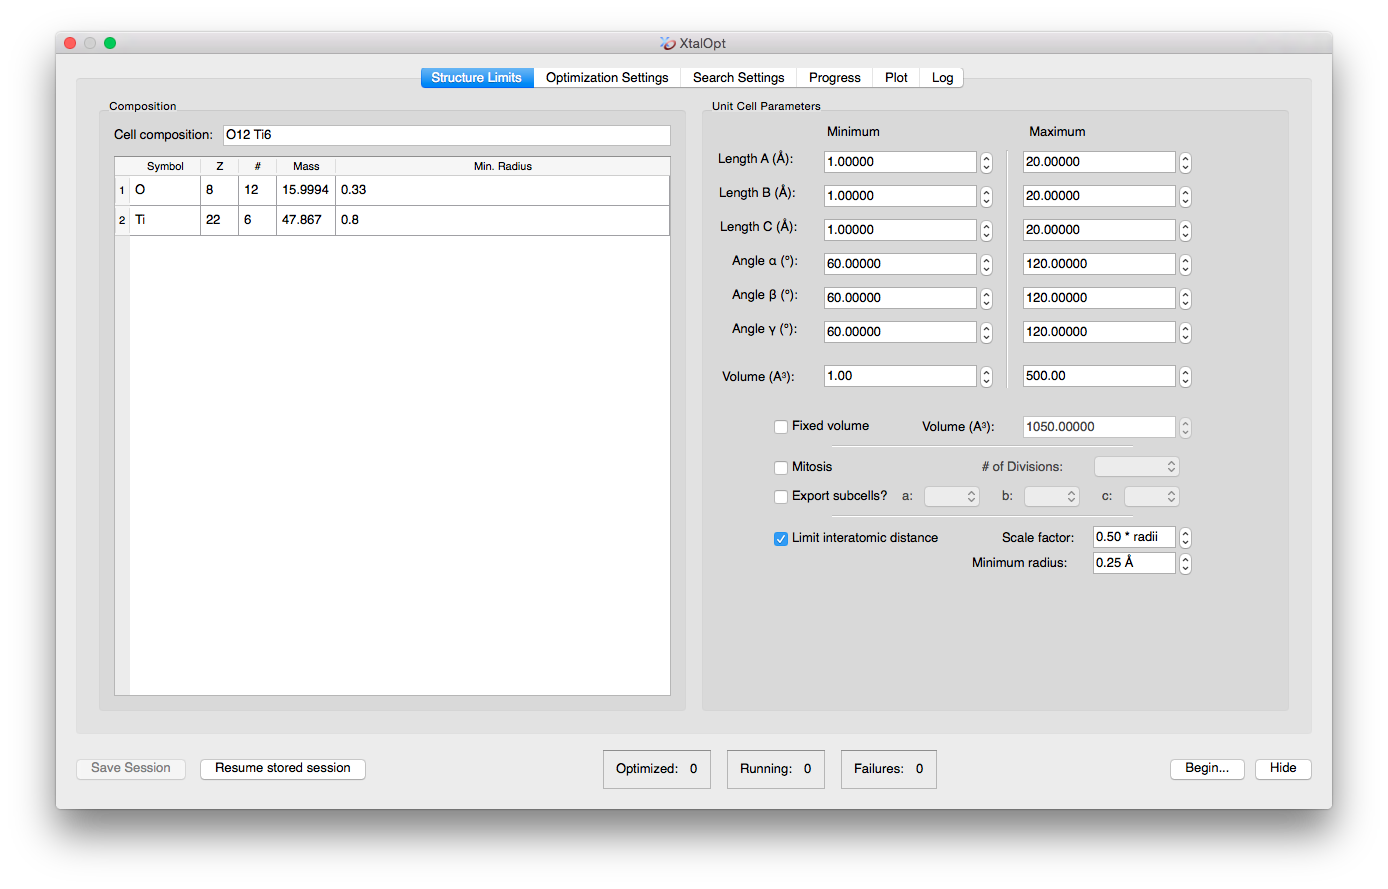
\includegraphics[width=\textwidth]{struct-lim.png}}
\end{DoxyImageNoCaption}


The interface opens to the \char`\"{}\+Structure Limits\char`\"{} tab, shown above. We will use a 6 formula unit supercell of titanium dioxide for this tutorial, so enter \char`\"{}\+Ti6 O12\char`\"{} for the cell composition. We will assume that we know nothing about the system and use very loose restraints. Set all cell length minima to 1 angstrom and maxima to 20 angstrom. Constrain the angles to be between 60 and 120 degrees, and the volume from between 1 and 500 cubic angstrom. Specify a minimum interatomic distance of 0.\+5 angstrom. (Note that due to the angle adjustment described in the C\+P\+C 2010 publication, 60-\/120 degrees is the largest range of cell angles that Xtal\+Opt will generate.)\hypertarget{tut-xo_opt}{}\section{Optimizer setup}\label{tut-xo_opt}
Xtal\+Opt currently supports the \hyperlink{tut-xo_vasp-opt}{V\+A\+S\+P}, \hyperlink{tut-xo_gulp-opt}{G\+U\+L\+P}, \hyperlink{tut-xo_pwscf-opt}{P\+Wscf}, \hyperlink{tut-xo_castep-opt}{C\+A\+S\+T\+E\+P}, and \hyperlink{tut-xo_siesta-opt}{S\+I\+E\+S\+T\+A} codes for performing geometry optimizations. Each is detailed in its own section below.\hypertarget{tut-xo_vasp-opt}{}\subsection{V\+A\+S\+P}\label{tut-xo_vasp-opt}
 
\begin{DoxyImageNoCaption}
  \mbox{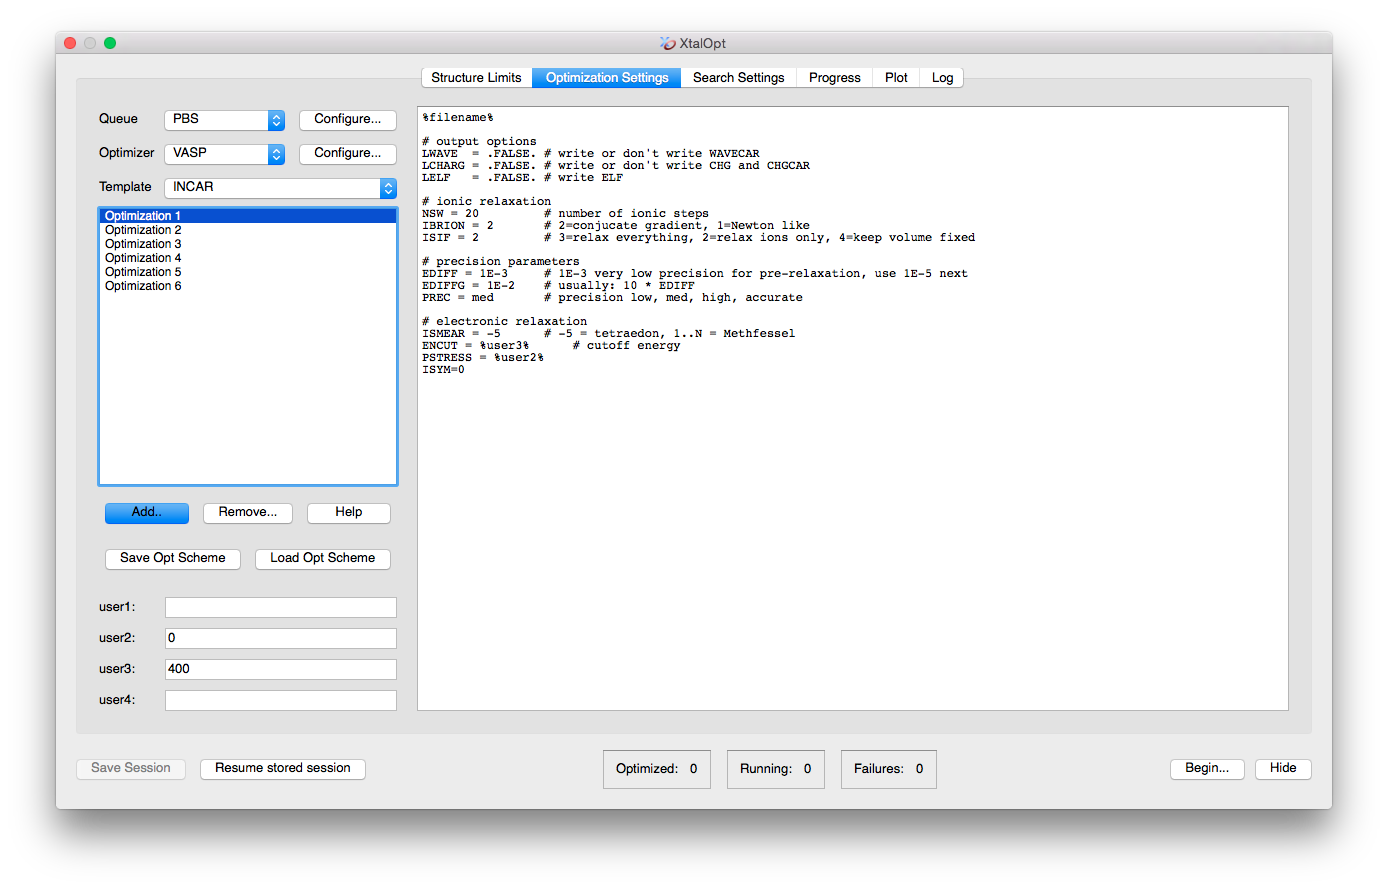
\includegraphics[width=\textwidth]{opt-set-vasp.png}}
\end{DoxyImageNoCaption}


On the next tab, load the optimization scheme by clicking the \char`\"{}\+Load
\+Opt Scheme\char`\"{} button and selecting the \char`\"{}samples/vasp-\/xtalopt.\+scheme\char`\"{} file that is distributed with the source code. If you do not have a copy of the source code, the scheme file can be obtained by clicking the \href{http://xtalopt.github.io/samples/vasp-xtalopt.scheme}{\tt here}.

For more details on optimization schemes, see \hyperlink{optschemes}{Optimization Schemes}.

After loading the optimization scheme, Xtal\+Opt will prompt for the P\+O\+T\+C\+A\+R files to use. Select files appropriated for the prompted atom. Xtal\+Opt will construct the P\+O\+T\+C\+A\+R files on the local computer, and then copy them over to the cluster when the calculation is submitted. It is necessary to have the V\+A\+S\+P P\+O\+T\+C\+A\+R files for each atomic species located somewhere on the local computer. See the V\+A\+S\+P manual for information on obtaining the P\+O\+T\+C\+A\+R files.

Take a moment to look through each file for each optimization step. Notice that the I\+N\+C\+A\+R template includes two user-\/specified values, \%user2\% and \%user3\% for the external pressure and the energy cutoff, respectively. By entering appropriate values in the \char`\"{}user2\+:\char`\"{} and \char`\"{}user3\+:\char`\"{} fields on the left, it is easy to update these values for all optimization steps.

Notice the other \%keyword\% values in the job.\+pbs templates. These are used to enter information that is specific to a search or structure when the actual input files are written prior to job submission. Click the \char`\"{}\+Help\char`\"{} button for a full listing of the available keywords.

Xtal\+Opt expects V\+A\+S\+P to use the default filenames, mainly P\+O\+S\+C\+A\+R, C\+O\+N\+T\+C\+A\+R, and O\+U\+T\+C\+A\+R.

\hyperlink{tut-xo_qisetup}{Skip to next section.}\hypertarget{tut-xo_gulp-opt}{}\subsection{G\+U\+L\+P}\label{tut-xo_gulp-opt}
 
\begin{DoxyImageNoCaption}
  \mbox{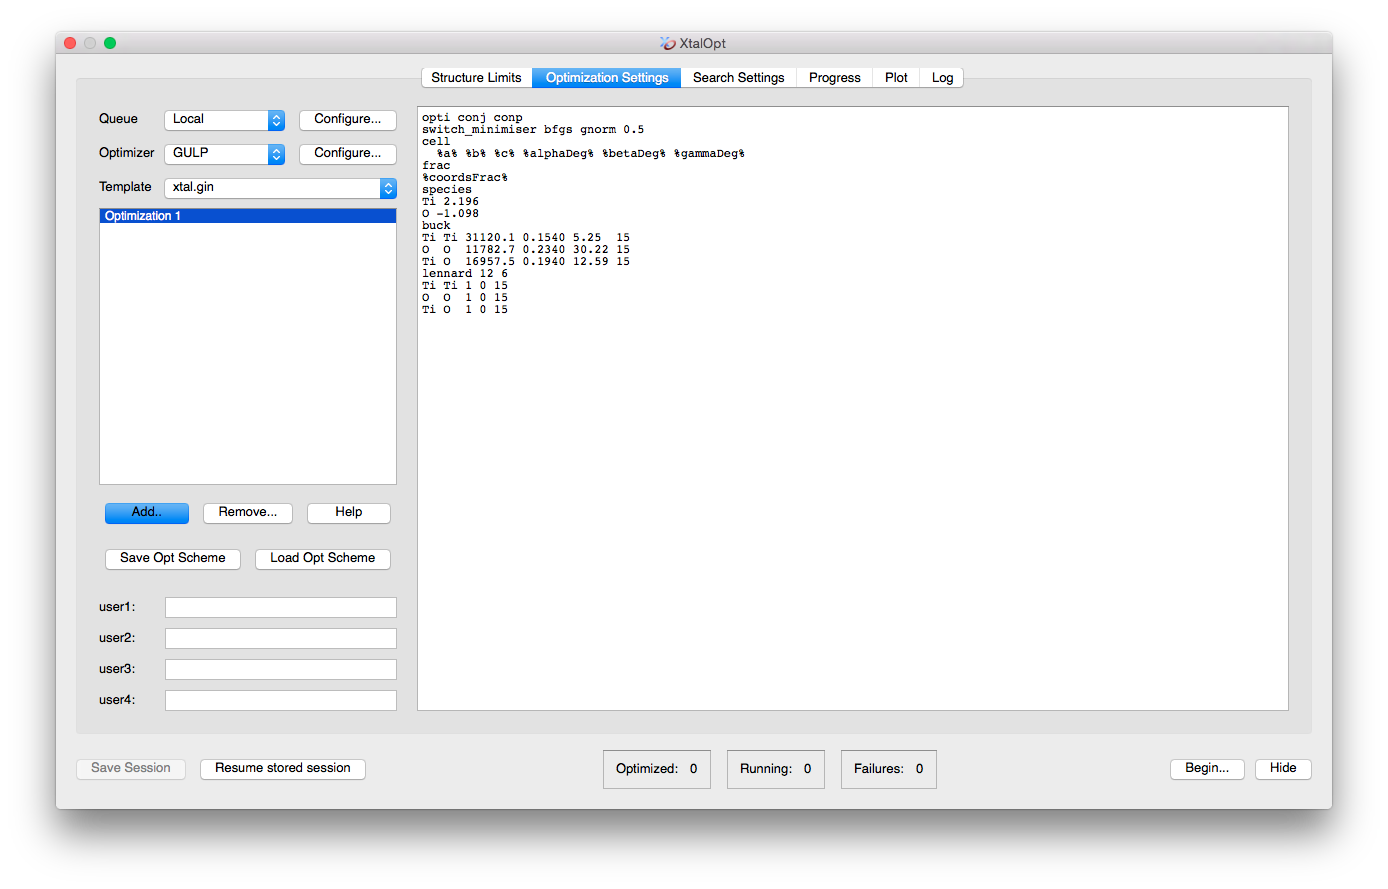
\includegraphics[width=\textwidth]{opt-set-gulp.png}}
\end{DoxyImageNoCaption}


On the next tab we choose G\+U\+L\+P for the local optimizer and enter a template for G\+U\+L\+P to use. Select \char`\"{}\+G\+U\+L\+P\char`\"{} as the \char`\"{}\+Optimizer\char`\"{} and \char`\"{}xtal.\+gin\char`\"{} as \char`\"{}\+Template\char`\"{}. Next, fill out the text field on the right with the following template\+: 
\begin{DoxyCode}
opti conj conp
switch\_minimiser bfgs gnorm 0.5
cell
  %a% %b% %c% %alphaDeg% %betaDeg% %gammaDeg%
frac
%coordsFrac%
species
Ti 2.196
O -1.098
buck
Ti Ti 31120.1 0.1540 5.25  15
O  O  11782.7 0.2340 30.22 15
Ti O  16957.5 0.1940 12.59 15
lennard 12 6
Ti Ti 1 0 15
O  O  1 0 15
Ti O  1 0 15
\end{DoxyCode}


Alternatively, one can load the scheme file distributed with the source code under samples/gulp-\/\+Ti\+O-\/xtalopt.\+scheme. If the source code is not available, the scheme file can be obtained by clicking \href{http://xtalopt.github.io/samples/gulp-TiO-xtalopt.scheme}{\tt here}.

For more details on optimization schemes, see \hyperlink{optschemes}{Optimization Schemes}.

Note the \char`\"{}\%\char`\"{} surrounding various keywords. These will be replaced by the structure-\/specific data when the optimizer is invoked for each structure. Click \char`\"{}\+Help\char`\"{} to view all of the keywords available. The number of optimization steps can be modified with the \char`\"{}\+Add/\+Resume\char`\"{} buttons. The \char`\"{}user\char`\"{} fields in the lower left corner allow users to specify their own keyword/value pairs, which is useful for making changes to multiple optimization steps at once. We will only be using one optimization step in this tutorial.

Xtal\+Opt expects G\+U\+L\+P to use the following filenames\+:


\begin{DoxyCode}
gulp < xtal.gin > xtal.got
\end{DoxyCode}


\hyperlink{tut-xo_qisetup}{Skip to next section.}\hypertarget{tut-xo_pwscf-opt}{}\subsection{P\+Wscf}\label{tut-xo_pwscf-opt}
 
\begin{DoxyImageNoCaption}
  \mbox{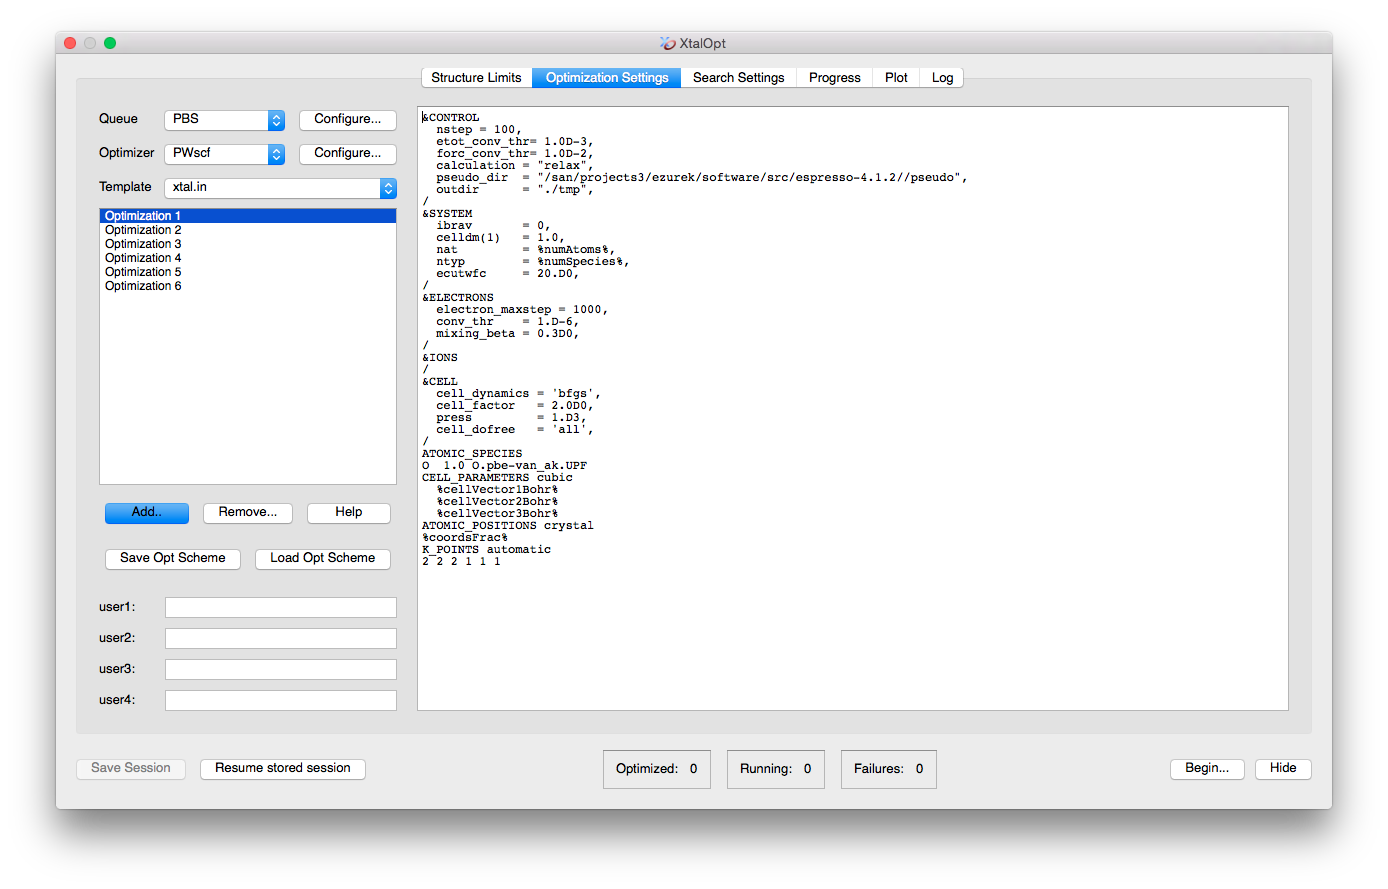
\includegraphics[width=\textwidth]{opt-set-pwscf.png}}
\end{DoxyImageNoCaption}


On the next tab, load the optimization scheme that is distributed with the source code under the samples/ directory. The scheme that we want is named \char`\"{}pwscf-\/xtalopt.\+scheme\char`\"{}. If the source code is not available, the scheme file can be obtained by clicking the \char`\"{}\+Original Format\char`\"{} link at the bottom of the page \href{http://xtalopt.github.io/samples/pwscf-xtalopt.scheme}{\tt here}.

For more details on optimization schemes, see \hyperlink{optschemes}{Optimization Schemes}.

Each P\+Wscf input file will need to be edited to specify\+:
\begin{DoxyEnumerate}
\item The pseudo\+\_\+dir containing the pseudopotential files on the remote cluster, and
\item The pseudopotentials for each atom (under A\+T\+O\+M\+I\+C\+\_\+\+S\+P\+E\+C\+I\+E\+S)
\end{DoxyEnumerate}

Take a moment to look through each file for each optimization step.

Notice the \%keyword\% values in the job.\+pbs templates. These are used to enter information that is specific to a search or structure when the actual input files are written prior to job submission. Click the \char`\"{}\+Help\char`\"{} button for a full listing of the available keywords.

Be aware that every P\+Wscf/\+C\+A\+S\+T\+E\+P installation is different, and it is almost certain that the job.\+pbs file included with this scheme will not work on any cluster other than the Zurek group\textquotesingle{}s \char`\"{}parity\char`\"{} cluster at S\+U\+N\+Y Buffalo\textquotesingle{}s Center for Computational Resources. It may take some experimentation to get jobs to submit successfully, and you may need to contact the mantainers of the cluster for assistance for information about M\+P\+I, executable locations, etc. Perhaps the easiest method to find the correct P\+B\+S script is to run some trial submissions by hand, and then replace the structure/search specific information with the appropriate keywords once a working script has been generated.

Xtal\+Opt expects P\+Wscf to use the following filenames\+:


\begin{DoxyCode}
pw.x < xtal.in > xtal.out
\end{DoxyCode}


\hyperlink{tut-xo_qisetup}{Skip to next section.}\hypertarget{tut-xo_castep-opt}{}\subsection{C\+A\+S\+T\+E\+P}\label{tut-xo_castep-opt}
 
\begin{DoxyImageNoCaption}
  \mbox{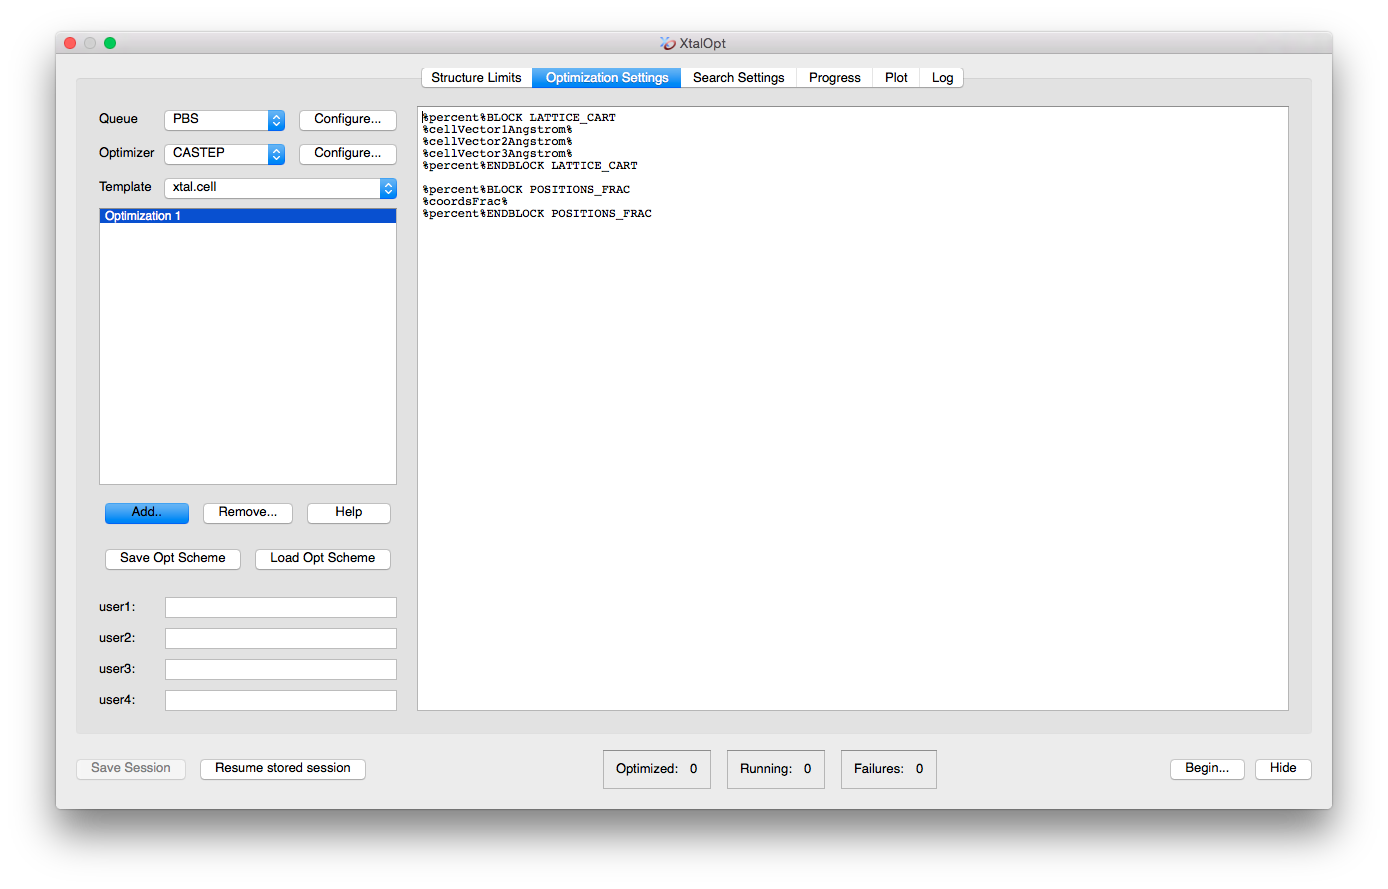
\includegraphics[width=\textwidth]{opt-set-castep.png}}
\end{DoxyImageNoCaption}


On the next tab, load the optimization scheme that is distributed with the source code under the samples/ directory. The scheme that we want is named \char`\"{}castep-\/xtalopt.\+scheme\char`\"{}. If the source code is not available, the scheme file can be obtained by clicking the \char`\"{}\+Original Format\char`\"{} link at the bottom of the page \href{http://xtalopt.github.io/samples/castep-xtalopt.scheme}{\tt here}.

For more details on optimization schemes, see \hyperlink{optschemes}{Optimization Schemes}.

It is important to note that C\+A\+S\+T\+E\+P input files require the \char`\"{}\%\char`\"{} character to define blocks. The percent character is special in the Xtal\+Opt input template parser to define keywords (see below). To insert a literal \char`\"{}\%\char`\"{} into the input, use percent\%.

E.\+g. Specification of the fractional coordinate block in the .cell template should look like\+:


\begin{DoxyCode}
%percent%BLOCK POSITIONS\_FRAC
%coordsFrac%
%percent%ENDBLOCK POSITIONS\_FRAC
\end{DoxyCode}


Take a moment to look through each file for each optimization step.

Notice the \%keyword\% values in the job.\+pbs templates. These are used to enter information that is specific to a search or structure when the actual input files are written prior to job submission. Click the \char`\"{}\+Help\char`\"{} button for a full listing of the available keywords.

Be aware that every P\+Wscf/\+C\+A\+S\+T\+E\+P installation is different, and it is almost certain that the job.\+pbs file included with this scheme will not work on any cluster other than the Zurek group\textquotesingle{}s \char`\"{}parity\char`\"{} cluster at S\+U\+N\+Y Buffalo\textquotesingle{}s Center for Computational Resources. It may take some experimentation to get jobs to submit successfully, and you may need to contact the mantainers of the cluster for assistance for information about M\+P\+I, executable locations, etc. Perhaps the easiest method to find the correct P\+B\+S script is to run some trial submissions by hand, and then replace the structure/search specific information with the appropriate keywords once a working script has been generated.

Xtal\+Opt expects C\+A\+S\+T\+E\+P to use the following filenames\+:


\begin{DoxyCode}
\textcolor{preprocessor}{# XtalOpt will write xtal.cell, xtal.param}
castep xtal
\textcolor{preprocessor}{# CASTEP will create xtal.castep}
\end{DoxyCode}


\hyperlink{tut-xo_qisetup}{Skip to next section.}\hypertarget{tut-xo_siesta-opt}{}\subsection{S\+I\+E\+S\+T\+A}\label{tut-xo_siesta-opt}
 
\begin{DoxyImageNoCaption}
  \mbox{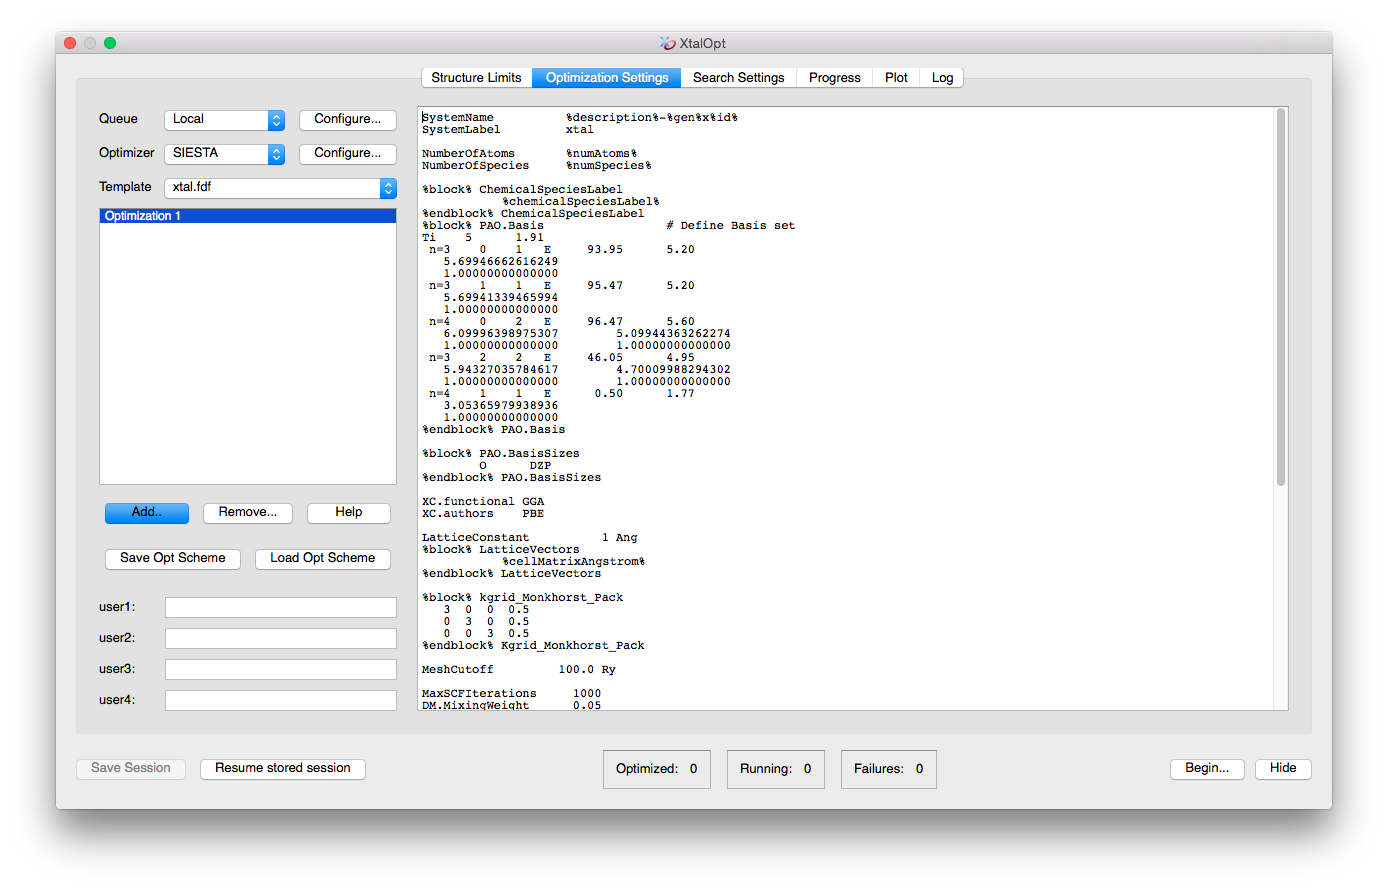
\includegraphics[width=\textwidth]{opt-set-siesta.png}}
\end{DoxyImageNoCaption}


On the next tab we choose G\+U\+L\+P for the local optimizer and enter a template for S\+I\+E\+S\+T\+A to use. Select \char`\"{}\+S\+I\+E\+S\+T\+A\char`\"{} as the \char`\"{}\+Optimizer\char`\"{} and \char`\"{}xtal.\+fdf\char`\"{} as \char`\"{}\+Template\char`\"{}.

Next, fill out the text field on the right with the following template\+:


\begin{DoxyCode}
SystemName          %description%-%gen%x%\textcolor{keywordtype}{id}%
SystemLabel         xtal

NumberOfAtoms       %numAtoms%
NumberOfSpecies     %numSpecies%

%block% ChemicalSpeciesLabel
%chemicalSpeciesLabel%
%endblock% ChemicalSpeciesLabel

%block% PAO.Basis                 # Define Basis set
Ti    5      1.91
 n=3    0    1   E     93.95      5.20
   5.69946662616249
   1.00000000000000
 n=3    1    1   E     95.47      5.20
   5.69941339465994
   1.00000000000000
 n=4    0    2   E     96.47      5.60
   6.09996398975307        5.09944363262274
   1.00000000000000        1.00000000000000
 n=3    2    2   E     46.05      4.95
   5.94327035784617        4.70009988294302
   1.00000000000000        1.00000000000000
 n=4    1    1   E      0.50      1.77
   3.05365979938936
   1.00000000000000
%endblock% PAO.Basis

%block% PAO.BasisSizes
        O      DZP
%endblock% PAO.BasisSizes

XC.functional GGA
XC.authors    PBE

LatticeConstant          1 Ang
%block% LatticeVectors
%cellMatrixAngstrom%
%endblock% LatticeVectors

%block% kgrid\_Monkhorst\_Pack
   3  0  0  0.5
   0  3  0  0.5
   0  0  3  0.5
%endblock% Kgrid\_Monkhorst\_Pack

MeshCutoff         100.0 Ry

MaxSCFIterations     1000
DM.MixingWeight      0.05
DM.NumberPulay       3
DM.Tolerance         1.d-4

SolutionMethod       diagon

SpinPolarized   \textcolor{keyword}{true}
LongOutput \textcolor{keyword}{true}

MD.TypeOfRun        cg
MD.NumCGsteps       1000
MD.VariableCell     \textcolor{keyword}{true}
MD.MaxForceTol      0.01 eV/Ang  #0.005 eV/Ang
WriteForces         \textcolor{keyword}{true}
WriteCoorCerius     \textcolor{keyword}{true}
WriteCoorXmol       \textcolor{keyword}{false}
WriteDenchar        \textcolor{keyword}{true}
WriteMullikenPop    1

UseSaveData         \textcolor{keyword}{true}

\textcolor{preprocessor}{#Diag.ParallelOverK true}

AtomicCoordinatesFormat Fractional
%block% AtomicCoordinatesAndAtomicSpecies
%atomicCoordsAndAtomicSpecies%
%endblock% AtomicCoordinatesAndAtomicSpecies
\end{DoxyCode}


Or load the optimization scheme by clicking the \char`\"{}\+Load Opt Scheme\char`\"{} button and selecting the \char`\"{}samples/siesta-\/\+Ti\+O-\/xtalopt.\+scheme\char`\"{} file that is distributed with the source code. If the source code is not available, the scheme file can be obtained by clicking \href{http://xtalopt.github.io/samples/siesta-TiO-xtalopt.scheme}{\tt here}.

For more details on optimization schemes, see \hyperlink{optschemes}{Optimization Schemes}.

After loading the optimization scheme, Xtal\+Opt will prompt for the xtal.\+psf files to use. Select files appropriated for the prompted atom. Xtal\+Opt will copy the individual files over to each structure directory when the calculation is submitted. See the S\+I\+E\+S\+T\+A manual for information on obtaining the .psf files.

Notice the other keyword\% values in the xtal.\+fdf templates. These are used to enter information that is specific to a search or structure when the actual input files are written prior to job submission. Click the \char`\"{}\+Help\char`\"{} button for a full listing of the available keywords.

Xtal\+Opt expects S\+I\+E\+S\+T\+A to use the following filenames\+:


\begin{DoxyPre}siesta < xtal.fdf > xtal.out\end{DoxyPre}
\hypertarget{tut-xo_qisetup}{}\section{Queue setup}\label{tut-xo_qisetup}
Xtal\+Opt currently supports using the \hyperlink{tut-xo_remotepbs}{P\+B\+S}, \hyperlink{tut-xo_remotesge}{S\+G\+E}, \hyperlink{tut-xo_remoteslurm}{S\+L\+U\+R\+M}, \hyperlink{tut-xo_remotelsf}{L\+S\+F}, and \hyperlink{tut-xo_remotell}{Load\+Leveler} queuing systems on remote S\+S\+H-\/accessible clusters, as well as an internal \hyperlink{tut-xo_localqi}{local} queue that manages calculations on the user\textquotesingle{}s workstation. Each queueing interface is detailed in its own section below.\hypertarget{tut-xo_remotepbs}{}\subsection{Using a remote P\+B\+S cluster}\label{tut-xo_remotepbs}
 
\begin{DoxyImageNoCaption}
  \mbox{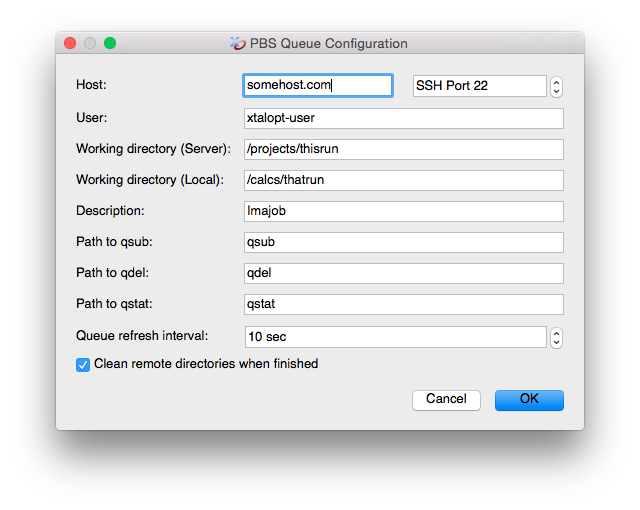
\includegraphics[width=\textwidth]{opt-set-pbs.png}}
\end{DoxyImageNoCaption}


Select \char`\"{}\+P\+B\+S\char`\"{} from the list of Queues, and then click the \char`\"{}\+Configure...\char`\"{} button. A new window will prompt for\+:
\begin{DoxyItemize}
\item host\+: The hostname of the P\+B\+S cluster\textquotesingle{}s head node
\item user\+: The username used to log into the cluster
\item Working directory (Server)\+: A directory that is readable/writable by \char`\"{}user\char`\"{} on the cluster, used when performing optimizations.
\item Working directory (Local)\+: A directory that is readable/writable by the current user on the local computer. This is where the final structures and resume files are written.
\item Description\+: Used for the \%description\% keyword in input templates.
\item Path to qsub\+: Where to find the qsub executable on the remote cluster. Note that if qsub is in the cluster\textquotesingle{}s \$\+P\+A\+T\+H, setting this to just \textquotesingle{}qsub\textquotesingle{} will work.
\item Path to qdel\+: Where to find the qdel executable on the remote cluster. Note that if qdel is in the cluster\textquotesingle{}s \$\+P\+A\+T\+H, setting this to just \textquotesingle{}qdel\textquotesingle{} will work.
\item Path to qstat\+: Where to find the qstat executable on the remote cluster. Note that if qstat is in the cluster\textquotesingle{}s \$\+P\+A\+T\+H, setting this to just \textquotesingle{}qstat\textquotesingle{} will work.
\end{DoxyItemize}

A new template, \char`\"{}job.\+pbs\char`\"{} is added to the list of available templates. This is the job submission script for P\+B\+S. This script should roughly follow this design\+:


\begin{DoxyCode}
\textcolor{preprocessor}{#/bin/bash}
\textcolor{preprocessor}{#PBS -l nodes=1:ppn=8}
\textcolor{preprocessor}{#PBS -o ../%gen%x%id%-%optstep%.out}
\textcolor{preprocessor}{#PBS -e ../%gen%x%id%-%optstep%.err}
\textcolor{preprocessor}{#PBS -N %description%-%gen%x%id%-%optstep%}

\textcolor{preprocessor}{###Include this for XtalOpt scripts!###}
export PBS\_O\_WORKDIR=%rempath%

\textcolor{preprocessor}{# Change to structure's working directory, copy input files to node's scratch dirs:}
\textcolor{keywordflow}{for} node in `cat $PBS\_NODEFILE | sort | uniq`; \textcolor{keywordflow}{do}
rsh $node \textcolor{stringliteral}{"cp $PBS\_O\_WORKDIR/* $PBSTMPDIR/;"};
done

\textcolor{preprocessor}{# Move to the scratch directory}
cd $PBSTMPDIR
echo \textcolor{stringliteral}{"running in directory $PBSTMPDIR"}

\textcolor{preprocessor}{# Set any environment variables needed for the optimizer/MPI here:}

\textcolor{preprocessor}{# Run optimizer, be sure to use the filenames that XtalOpt expects.}
\textcolor{preprocessor}{# See the template menu in XtalOpt and the example templates in the}
\textcolor{preprocessor}{# samples/ directory of the XtalOpt sources.}

\textcolor{preprocessor}{# Don't forget to clean up after MPI if needed!}

\textcolor{comment}{// Print files from each node}
\textcolor{keywordflow}{for} node in `cat $PBS\_NODEFILE | sort | uniq`; \textcolor{keywordflow}{do}
echo \textcolor{stringliteral}{"$node:"}
rsh $node \textcolor{stringliteral}{"ls -l $PBSTMPDIR"}
done
\textcolor{preprocessor}{# Copy back results from master node's scratch directory}
\textcolor{preprocessor}{cp $PBSTMPDIR}\textcolor{comment}{/* $PBS\_O\_WORKDIR/}
\end{DoxyCode}


For more details on optimization schemes, see \hyperlink{optschemes}{Optimization Schemes}.

Be aware that every installation is different, and it is almost certain that the job.\+pbs file included with this scheme will not work on any cluster other than the Zurek group\textquotesingle{}s \char`\"{}parity\char`\"{} cluster at S\+U\+N\+Y Buffalo\textquotesingle{}s Center for Computational Resources. It may take some experimentation to get jobs to submit successfully, and you may need to contact the mantainers of the cluster for assistance or information about M\+P\+I, executable locations, etc. Perhaps the easiest method to find the correct P\+B\+S script is to run some trial submissions by hand, and then replace the structure/search specific information with the appropriate keywords once a working script has been generated.

A handy trick for monitoring jobs outside of Xtal\+Opt is to include the following line in job.\+pbs\+:


\begin{DoxyCode}
\textcolor{preprocessor}{#PBS -N %description%-%gen%x%id%-%optstep%}
\end{DoxyCode}


This will name each job, for example, xtal\+Search-\/3x4-\/2, where xtal\+Search is a user-\/specified description of the search, and 3x4-\/2 means that it is the fourth structure in the third generation running its second optimization step.

\hyperlink{tut-xo_files}{Skip to next section.}\hypertarget{tut-xo_remotesge}{}\subsection{Using a remote S\+G\+E cluster}\label{tut-xo_remotesge}
 
\begin{DoxyImageNoCaption}
  \mbox{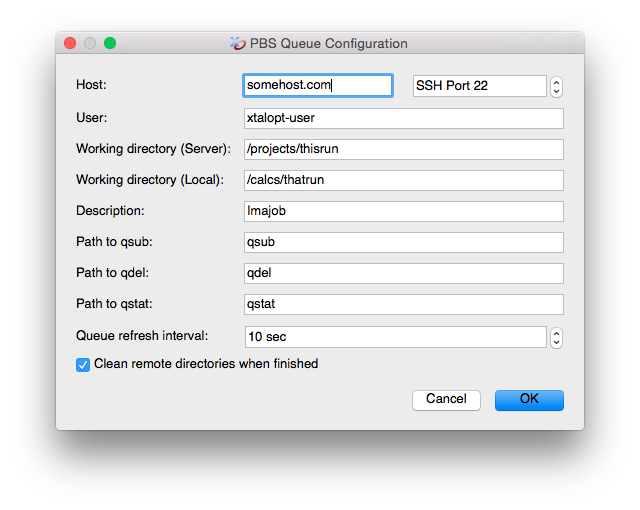
\includegraphics[width=\textwidth]{opt-set-pbs.png}}
\end{DoxyImageNoCaption}
 \begin{DoxyRefDesc}{Todo}
\item[\hyperlink{todo__todo000001}{Todo}]Get screenshots of S\+G\+E config dialog\end{DoxyRefDesc}


Select \char`\"{}\+S\+G\+E\char`\"{} from the list of Queues, and then click the \char`\"{}\+Configure...\char`\"{} button. A new window will prompt for\+:
\begin{DoxyItemize}
\item host\+: The hostname of the S\+G\+E cluster\textquotesingle{}s head node
\item user\+: The username used to log into the cluster
\item Working directory (Server)\+: A directory that is readable/writable by \char`\"{}user\char`\"{} on the cluster, used when performing optimizations.
\item Working directory (Local)\+: A directory that is readable/writable by the current user on the local computer. This is where the final structures and resume files are written.
\item Description\+: Used for the \%description\% keyword in input templates.
\item Path to qsub\+: Where to find the qsub executable on the remote cluster. Note that if qsub is in the cluster\textquotesingle{}s \$\+P\+A\+T\+H, setting this to just \textquotesingle{}qsub\textquotesingle{} will work.
\item Path to qdel\+: Where to find the qdel executable on the remote cluster. Note that if qdel is in the cluster\textquotesingle{}s \$\+P\+A\+T\+H, setting this to just \textquotesingle{}qdel\textquotesingle{} will work.
\item Path to qstat\+: Where to find the qstat executable on the remote cluster. Note that if qstat is in the cluster\textquotesingle{}s \$\+P\+A\+T\+H, setting this to just \textquotesingle{}qstat\textquotesingle{} will work.
\end{DoxyItemize}

\begin{DoxyRefDesc}{Todo}
\item[\hyperlink{todo__todo000002}{Todo}]Get template for job.\+sge scripts\end{DoxyRefDesc}


A new template, \char`\"{}job.\+sge\char`\"{} is added to the list of available templates. This is the job submission script for S\+G\+E. It may take some experimentation to get jobs to submit successfully, and you may need to contact the mantainers of the cluster for assistance or information about M\+P\+I, executable locations, etc. Perhaps the easiest method to find the correct S\+G\+E script is to run some trial submissions by hand, and then replace the structure/search specific information with the appropriate keywords once a working script has been generated.

For more details on optimization schemes, see \hyperlink{optschemes}{Optimization Schemes}.

\hyperlink{tut-xo_files}{Skip to next section.}\hypertarget{tut-xo_remoteslurm}{}\subsection{Using a remote S\+L\+U\+R\+M cluster}\label{tut-xo_remoteslurm}
 
\begin{DoxyImageNoCaption}
  \mbox{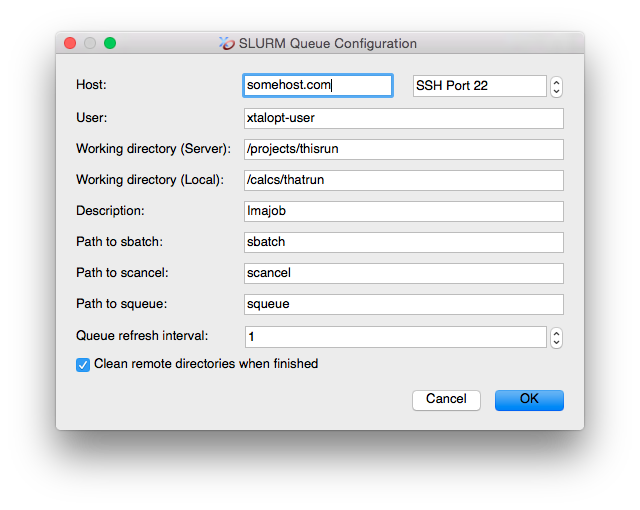
\includegraphics[width=\textwidth]{opt-set-slurm.png}}
\end{DoxyImageNoCaption}


Select \char`\"{}\+S\+L\+U\+R\+M\char`\"{} from the list of Queues, and then click the \char`\"{}\+Configure...\char`\"{} button. A new window will prompt for\+:
\begin{DoxyItemize}
\item host\+: The hostname of the S\+G\+E cluster\textquotesingle{}s head node
\item user\+: The username used to log into the cluster
\item Working directory (Server)\+: A directory that is readable/writable by \char`\"{}user\char`\"{} on the cluster, used when performing optimizations.
\item Working directory (Local)\+: A directory that is readable/writable by the current user on the local computer. This is where the final structures and resume files are written.
\item Description\+: Used for the \%description\% keyword in input templates.
\item Path to sbatch\+: Where to find the sbatch executable on the remote cluster. Note that if sbatch is in the cluster\textquotesingle{}s \$\+P\+A\+T\+H, setting this to just \textquotesingle{}sbatch\textquotesingle{} will work.
\item Path to scancel\+: Where to find the scancel executable on the remote cluster. Note that if scancel is in the cluster\textquotesingle{}s \$\+P\+A\+T\+H, setting this to just \textquotesingle{}scancel\textquotesingle{} will work.
\item Path to squeue\+: Where to find the squeue executable on the remote cluster. Note that if squeue is in the cluster\textquotesingle{}s \$\+P\+A\+T\+H, setting this to just \textquotesingle{}squeue\textquotesingle{} will work.
\end{DoxyItemize}

\begin{DoxyRefDesc}{Todo}
\item[\hyperlink{todo__todo000003}{Todo}]Get template for job.\+slurm scripts\end{DoxyRefDesc}


A new template, \char`\"{}job.\+slurm\char`\"{} is added to the list of available templates. This is the job submission script for S\+L\+U\+R\+M. It may take some experimentation to get jobs to submit successfully, and you may need to contact the mantainers of the cluster for assistance or information about M\+P\+I, executable locations, etc. Perhaps the easiest method to find the correct S\+L\+U\+R\+M script is to run some trial submissions by hand, and then replace the structure/search specific information with the appropriate keywords once a working script has been generated.

For more details on optimization schemes, see \hyperlink{optschemes}{Optimization Schemes}.

\hyperlink{tut-xo_files}{Skip to next section.}\hypertarget{tut-xo_remotelsf}{}\subsection{Using a remote L\+S\+F cluster}\label{tut-xo_remotelsf}
 
\begin{DoxyImageNoCaption}
  \mbox{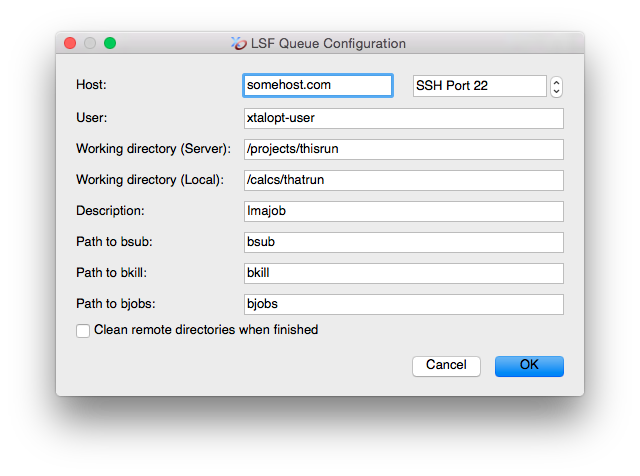
\includegraphics[width=\textwidth]{opt-set-lsf.png}}
\end{DoxyImageNoCaption}


Select \char`\"{}\+L\+S\+F\char`\"{} from the list of Queues, and then click the \char`\"{}\+Configure...\char`\"{} button. A new window will prompt for\+:
\begin{DoxyItemize}
\item host\+: The hostname of the L\+S\+F cluster\textquotesingle{}s head node
\item user\+: The username used to log into the cluster
\item Working directory (Server)\+: A directory that is readable/writable by \char`\"{}user\char`\"{} on the cluster, used when performing optimizations.
\item Working directory (Local)\+: A directory that is readable/writable by the current user on the local computer. This is where the final structures and resume files are written.
\begin{DoxyItemize}
\item Description\+: Used for the description\% keyword in input templates.
\item Path to bsub\+: Where to find the bsub executable on the remote cluster. Note that if bsub is in the cluster\textquotesingle{}s \$\+P\+A\+T\+H, setting this to just \textquotesingle{}bsub\textquotesingle{} will work.
\item Path to bkill\+: Where to find the bkill executable on the remote cluster. Note that if bkill is in the cluster\textquotesingle{}s \$\+P\+A\+T\+H, setting this to just \textquotesingle{}bkill\textquotesingle{} will work.
\item Path to bjobs\+: Where to find the bjobs executable on the remote cluster. Note that if bjobs is in the cluster\textquotesingle{}s \$\+P\+A\+T\+H, setting this to just \textquotesingle{}bjobs\textquotesingle{} will work.
\end{DoxyItemize}
\end{DoxyItemize}

A new template, \char`\"{}job.\+lsf\char`\"{} is added to the list of available templates. This is the job submission script for L\+S\+F. It may take some experimentation to get jobs to submit successfully, and you may need to contact the mantainers of the cluster for assistance or information about M\+P\+I, executable locations, etc. Perhaps the easiest method to find the correct L\+S\+F script is to run some trial submissions by hand, and then replace the structure/search specific information with the appropriate keywords once a working script has been generated.

For more details on optimization schemes, see \hyperlink{optschemes}{Optimization Schemes}.

\hyperlink{tut-xo_files}{Skip to next section.}\hypertarget{tut-xo_remotell}{}\subsection{Using a remote Load\+Leveler cluster}\label{tut-xo_remotell}
 
\begin{DoxyImageNoCaption}
  \mbox{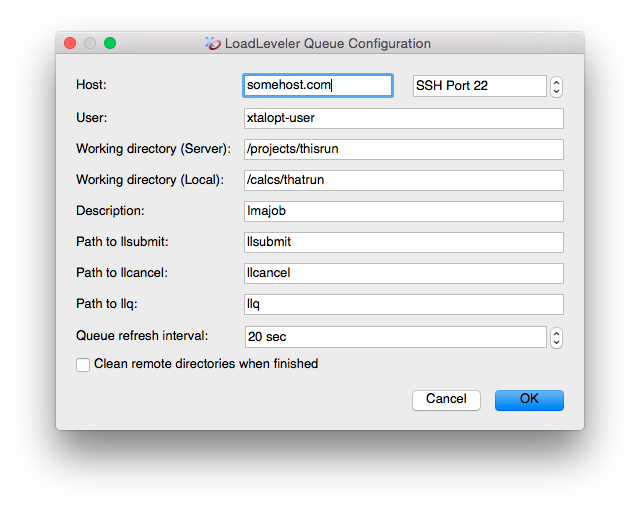
\includegraphics[width=\textwidth]{opt-set-ll.png}}
\end{DoxyImageNoCaption}


Select \char`\"{}\+Load\+Leveler\char`\"{} from the list of Queues, and then click the \char`\"{}\+Configure...\char`\"{} button. A new window will prompt for\+:
\begin{DoxyItemize}
\item host\+: The hostname of the Load\+Leveler cluster\textquotesingle{}s head node
\item user\+: The username used to log into the cluster
\item Working directory (Server)\+: A directory that is readable/writable by \char`\"{}user\char`\"{} on the cluster, used when performing optimizations.
\item Working directory (Local)\+: A directory that is readable/writable by the current user on the local computer. This is where the final structures and resume files are written.
\item Description\+: Used for the description\% keyword in input templates.
\item Path to llsubmit\+: Where to find the llsubmit executable on the remote cluster. Note that if llsubmit is in the cluster\textquotesingle{}s \$\+P\+A\+T\+H, setting this to just \textquotesingle{}llsubmit\textquotesingle{} will work.
\item Path to llcancel\+: Where to find the llcancel executable on the remote cluster. Note that if llcancel is in the cluster\textquotesingle{}s \$\+P\+A\+T\+H, setting this to just \textquotesingle{}llcancel\textquotesingle{} will work.
\item Path to llq\+: Where to find the llq executable on the remote cluster. Note that if llq is in the cluster\textquotesingle{}s \$\+P\+A\+T\+H, setting this to just \textquotesingle{}llq\textquotesingle{} will work.
\end{DoxyItemize}

A new template, \char`\"{}job.\+ll\char`\"{} is added to the list of available templates. This is the job submission script for Load\+Leveler. It may take some experimentation to get jobs to submit successfully, and you may need to contact the mantainers of the cluster for assistance or information about M\+P\+I, executable locations, etc. Perhaps the easiest method to find the correct Load\+Leveler script is to run some trial submissions by hand, and then replace the structure/search specific information with the appropriate keywords once a working script has been generated.

For more details on optimization schemes, see \hyperlink{optschemes}{Optimization Schemes}.

\hyperlink{tut-xo_files}{Skip to next section.}\hypertarget{tut-xo_localqi}{}\subsection{Running optimations locally}\label{tut-xo_localqi}
 
\begin{DoxyImageNoCaption}
  \mbox{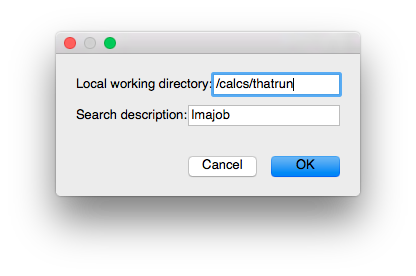
\includegraphics[width=.5\textwidth]{opt-set-local.png}}
\end{DoxyImageNoCaption}


Select \char`\"{}\+Local\char`\"{} from the list of Queues, and then click the configure button. A new window will prompt for\+:
\begin{DoxyItemize}
\item Local working directory\+: A directory that is readable/writable by the current user on the local computer. This is where the final structures and resume files are written.
\end{DoxyItemize}

If the optimizer\textquotesingle{}s executable (vasp, gulp, pw.\+x, castep, etc) is not in your system path, you will need to specify the location of the executable by clicking the \char`\"{}\+Configure...\char`\"{} button next to the optimizer selection menu.

For more details on optimization schemes, see \hyperlink{optschemes}{Optimization Schemes}.\hypertarget{tut-xo_files}{}\section{What is written to the local directory?}\label{tut-xo_files}
A directory for each structure is created at


\begin{DoxyCode}
[Local working directory]/<gen#>x<id#>
\end{DoxyCode}


that will contain input, output, and data files specific to each structure. Two additional files are also written to the local filesystem\+:


\begin{DoxyCode}
[Local working directory]/xtalopt.state
\end{DoxyCode}


which contains save/resume information to continue a session that has been stopped, and


\begin{DoxyCode}
[Local working directory]/results.txt
\end{DoxyCode}


which stores a list of all structures sorted by increasing enthalpy. The latter file is handy for offline analysis, since there is no need to open Xtal\+Opt to find the most stable structures of a previous search.\hypertarget{tut-xo_search-set}{}\section{Search Settings}\label{tut-xo_search-set}
 
\begin{DoxyImageNoCaption}
  \mbox{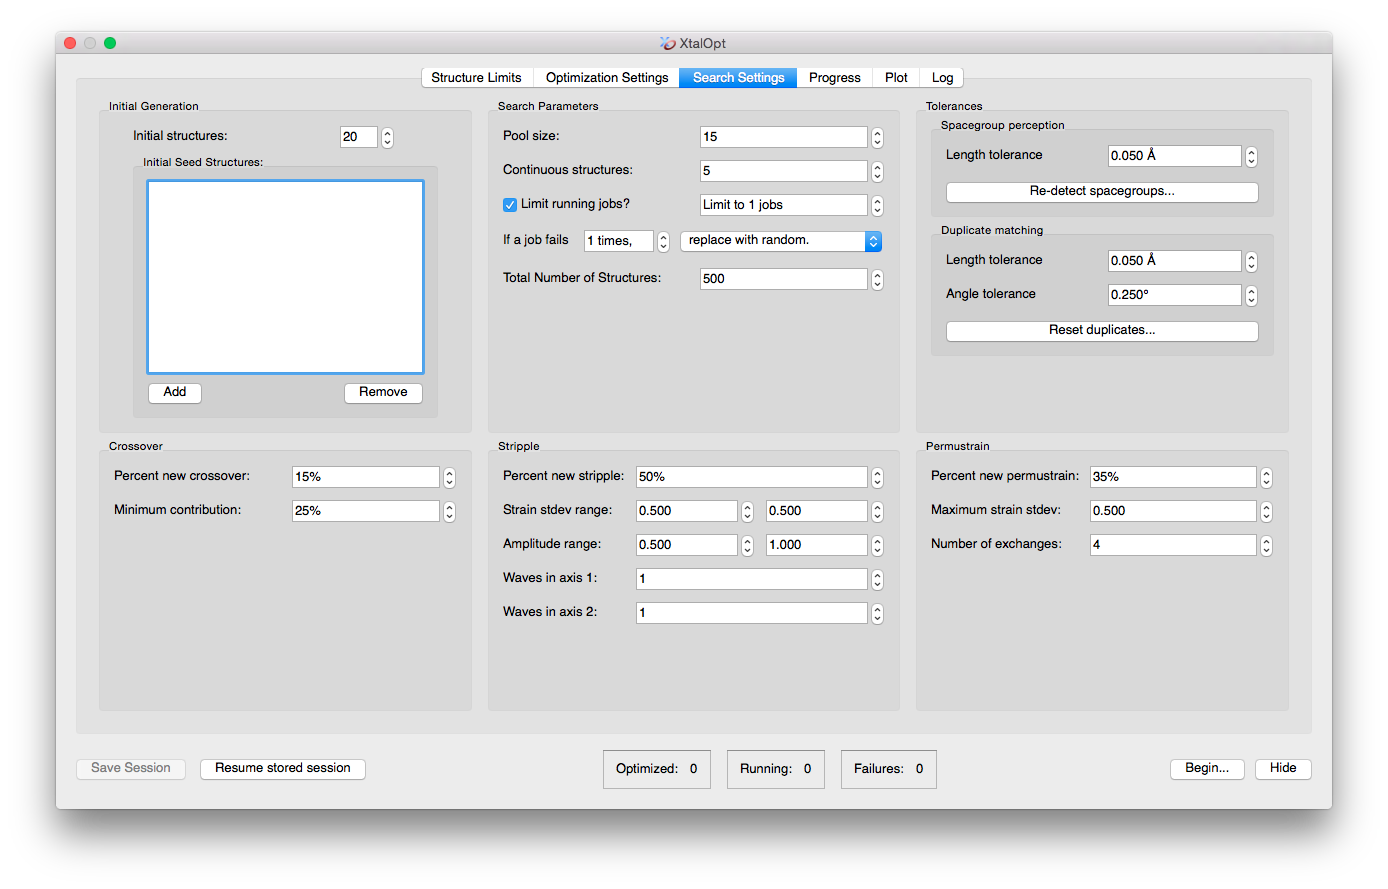
\includegraphics[width=\textwidth]{search-set.png}}
\end{DoxyImageNoCaption}


In the \char`\"{}\+Search Settings\char`\"{} tab, most of the default settings should suffice (See C\+P\+C 2010 publication). We arbitrarily set the initial structures to 20 and the continuous structures to 5, although these may need to be adjusted based on available resources. We will not specify initial seeds, but the option to do so exists on this screen.

It is not neccessary to limit the number of running jobs unless running locally, as the P\+B\+S queue on the cluster will manage job control for us. If running locally, set the job limit no higher than \mbox{[}number of available processor cores\mbox{]} -\/ 1 (e.\+g. for a quadcore processor, allow three jobs to run simultaneously). This allows one core to remain free for the system to run.

There is now a termination criteria called \char`\"{}\+Total Number of Structures\char`\"{} that will end the run once a certain number of strcutures have been produced by Xtal\+Opt.\hypertarget{tut-xo_begin}{}\section{\char`\"{}\+Begin\char`\"{}}\label{tut-xo_begin}

\begin{DoxyImage}
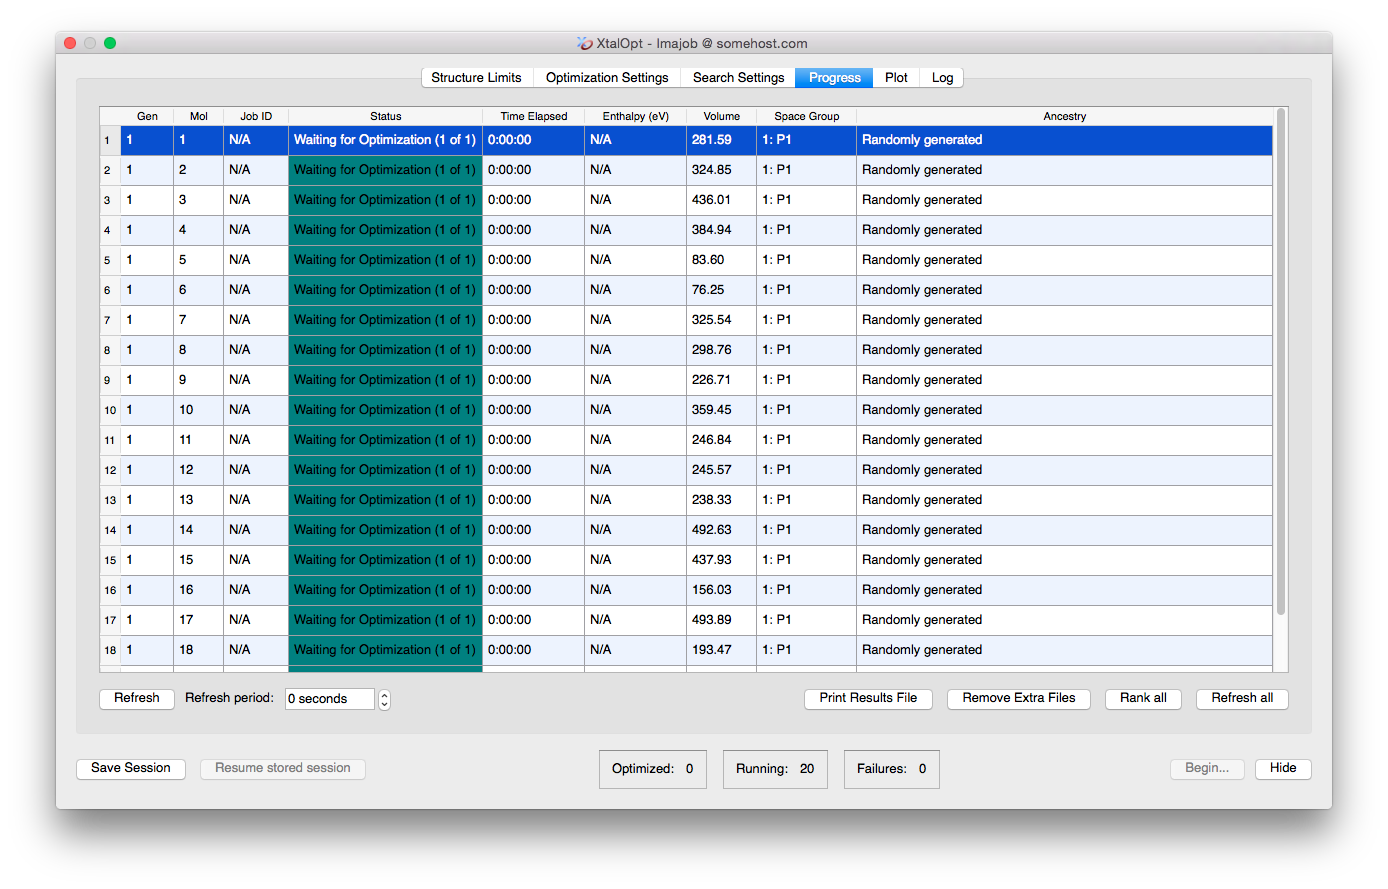
\includegraphics[width=\textwidth]{prog-start.png}
\caption{The ``\+Progress\textquotesingle{}\textquotesingle{} tab immediately after starting a search}
\end{DoxyImage}


Xtal\+Opt has everything it needs to start its search at this point; click the \char`\"{}\+Begin\char`\"{} button in the lower right corner of the application to tell it to start the search algorithm. A progress bar appears as the random first generation is created. Switch to the \char`\"{}\+Progress\char`\"{} tab and 20 entries will appear, all with a status of \char`\"{}\+Waiting for
\+Optimization\char`\"{}. Click \char`\"{}\+Refresh\char`\"{} on this tab to begin the local optimizations. From here, Xtal\+Opt will continue to run without user input, starting new optimizations and generating new structures until it is stopped by the user.\hypertarget{tut-xo_prog-mon}{}\section{Monitor progress}\label{tut-xo_prog-mon}

\begin{DoxyImage}
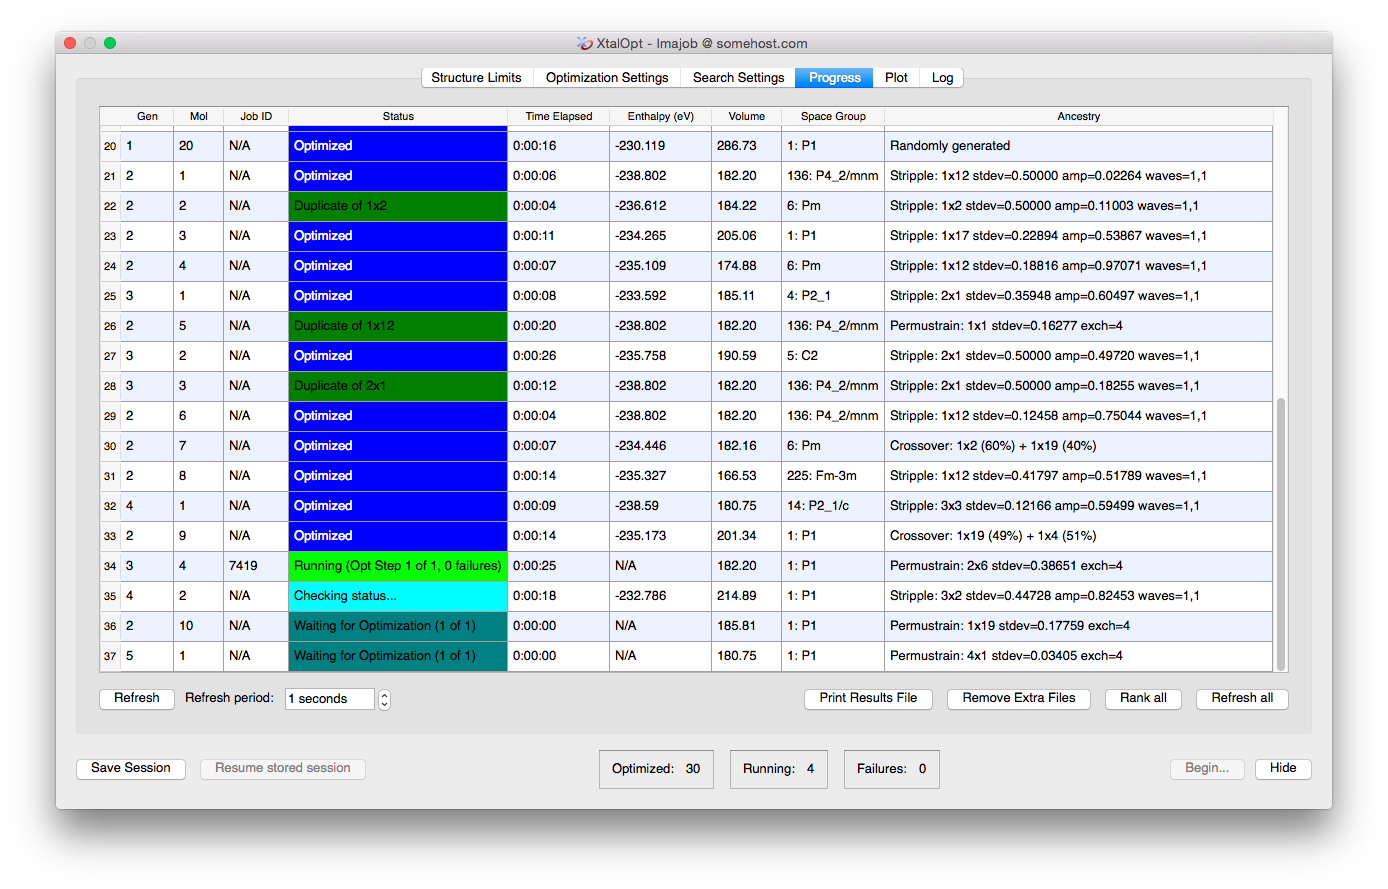
\includegraphics[width=\textwidth]{prog-mon.png}
\caption{The ``\+Progress\textquotesingle{}\textquotesingle{} tab mid-\/run}
\end{DoxyImage}


As Xtal\+Opt performs the search, the progress table continuously updates, providing information about each structure. We see individuals in various stages of completion\+: most are optimized (in blue), structure 2x7 has been automatically marked as a duplicate (dark green) of structure 3x3 and removed from the breeding pool, structure 4x4 is currently undergoing a local optimization (light green), while structure 4x5 is waiting to be optimized (light blue).

Other useful information is displayed about each structure, such as the time spent in optimization, the optimized enthalpy, the cell volume, spacegroup, and each structure\textquotesingle{}s ancestory (i.\+e. parent(s) and parameters for the genetic operator that generated it). A status bar on the bottom of the window shows the number of structures that are optimized, running, and failing at any given time. This information is visible regardless of which tab is currently being viewed.

An additional feature of the progress table is the ability to immediately visualize any of the individuals in the Avogadro main window -- simply clicking on a row in this table will display the three-\/dimensional structure in Avogadro, where it can be visualized, modified, or exported. If the user would like to add a bit of \char`\"{}intelligent design\char`\"{} to the evolutionary process, a structure can be modified and then resubmitted using a context (right-\/click) menu from the progress table. The context menu provides tools to (un)kill a structure, resubmit for local optimization at an arbitrary optimization step, or replace a problematic structure with a new, random individual.

Three additional buttons found near the \char`\"{}\+Refresh All\char`\"{} button in this tab are also available. The \char`\"{}\+Print Results File\char`\"{} button generates a run-\/results.\+txt file that lists all of the information about each structure in order of generation and structure number (As compared to the results.\+txt file which ranks the structures). The \char`\"{}\+Remove Extra Files\char`\"{} button is used for V\+A\+S\+P runs. It removes any extraneous files in each local subdirectory in order to reduce disk usage. Files kept are structure.\+state, P\+O\+T\+C\+A\+R, C\+O\+N\+T\+C\+A\+R, O\+S\+Z\+I\+C\+A\+R, job.\+slurm and O\+U\+T\+C\+A\+R. Finally, the \char`\"{}\+Rank All\char`\"{} button ranks all currently optimized structures and exports them to a subdirectory (Ranked) in two forms (depending on the optimizer)\+: P\+O\+S\+C\+A\+R/.got and .cif. Each can be found in separate directories. (Only works for G\+U\+L\+P and V\+A\+S\+P runs currently).\hypertarget{tut-xo_trends}{}\subsection{View trends}\label{tut-xo_trends}

\begin{DoxyImage}
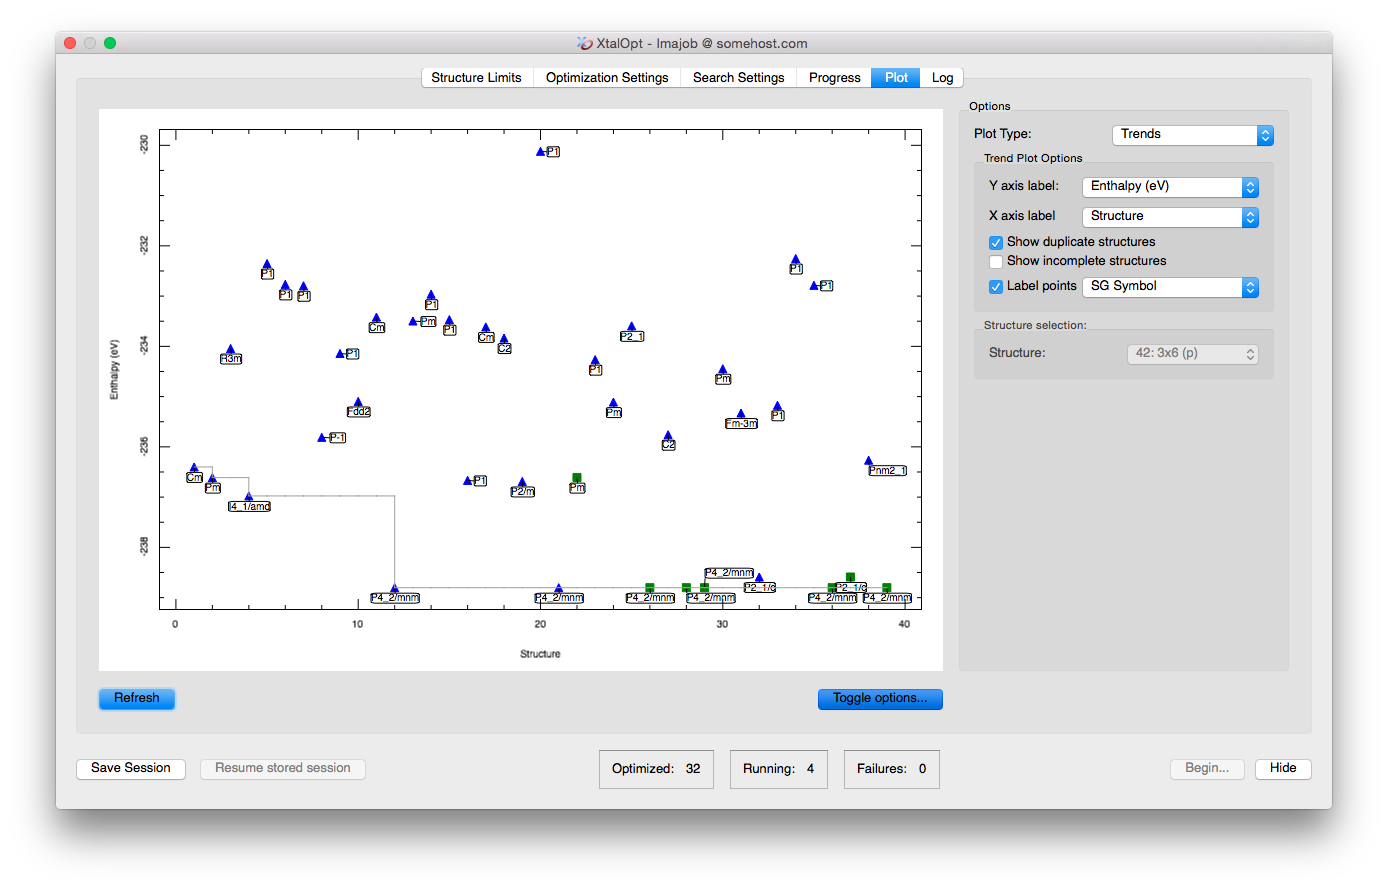
\includegraphics[width=\textwidth]{trend-view.png}
\caption{The ``\+Plot\textquotesingle{}\textquotesingle{} tab mid-\/run displaying enthalpy vs. volume. Each structure is labeled with its Hermann Mauguin spacegroup symbol.}
\end{DoxyImage}


Another visualization and analysis tool available during the search is the interactive plot. The plot is capable of investigating trends in the search by plotting a point for each individual using structure number, generation number, enthalpy, energy, \$\+P\+V\$ enthalpy term, lattice parameters, or cell volume on either axis. This powerful feature allows the user to visualize complex relationships present in the generated structures. E.\+g., a plot of enthalpy vs. structure number provides an overview of the search\textquotesingle{}s progress. Or, recalling that H = U + P\+V, plotting enthalpy vs. P\+V enthalpy term or energy lends insight into whether the enthalpy (H) is dominated by atomic interactions (U) or cell parameters (P\+V). Further information is available by labeling the points with the individual\textquotesingle{}s spacegroup number, Hermann Mauguin spacegroup symbol, enthalpy, energy, P\+V term, volume, generation, or index number.

A particularly useful plot is that of enthalpy vs. cell volume, as shown above. From this view, we see a general trend that enthalpy increases with volume (the effect is much more pronounced for systems at higher pressures), and also that below a certain volume enthalpy rises sharply. From this data set, we see that there is a cluster of very low enthalpy structures with cell volumes around 180 cubic angstroms. Armed with this data, we can update the starting volume on the Cell Initialization tab mid-\/run to reflect this new piece of information that the search has provided us. Many of the other parameters governing structure generation and algorithm specifics can be similarly modified during a search without the need to restart the algorithm.

The plot is also interactive; zooming and panning are possible using simple mouse controls. Clicking on a structure\textquotesingle{}s point on the plot will load it in the main Avogadro window, allow all the same functionality as described above in \hyperlink{tut-xo_prog-mon}{Monitor progress}. 
\section{Saving and Resuming Sessions in Xtal\+Opt}
\label{xo_saveresume}
\hypertarget{xo_saveresume}{}
\hypertarget{xo_saveresume_sr_contents}{}\section{Contents}\label{xo_saveresume_sr_contents}

\begin{DoxyItemize}
\item \hyperlink{xo_saveresume_sr_saving}{How to save your session}
\item \hyperlink{xo_saveresume_sr_resuming}{How to resume your session}
\end{DoxyItemize}

 
\begin{DoxyImageNoCaption}
  \mbox{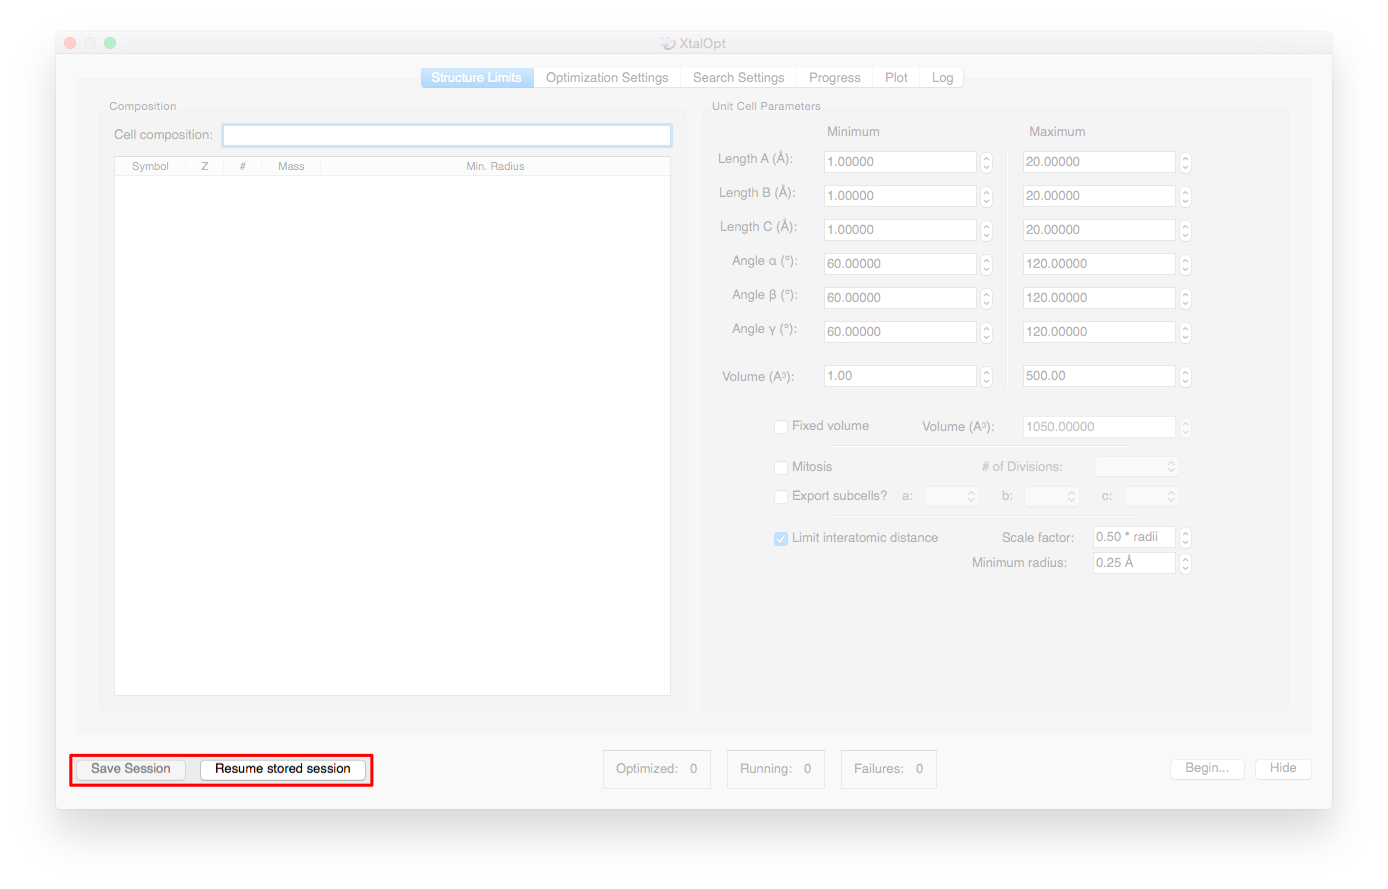
\includegraphics[width=\textwidth]{xo-saveresume.png}}
\end{DoxyImageNoCaption}
\hypertarget{xo_saveresume_sr_saving}{}\section{How to save your session}\label{xo_saveresume_sr_saving}
Xtal\+Opt will write a small file named xtalopt.\+state to its working directory that contains the information necessary to resume the session at a later time. The file can be rewritten manually by clicking the \char`\"{}\+Save Session\char`\"{} button highlighted above, and Xtal\+Opt will automatically save the session every time a structure is updated.

Xtal\+Opt will also write a file \char`\"{}structure.\+state\char`\"{} in each candidate structure\textquotesingle{}s directory. This file stores Xtal\+Opt-\/specific information about the structure.\hypertarget{xo_saveresume_sr_resuming}{}\section{How to resume your session}\label{xo_saveresume_sr_resuming}
To resume a session, simply click \char`\"{}\+Resume stored session\char`\"{} (highlighted above) and select the xtalopt.\+state file in the working directory of the session you would like to resume. Xtal\+Opt will then begin to load the structures and search parameters. You can monitor the progress with the progress bar that appears at the bottom of the window.

While the structures are loading, you may encounter errors that say\+:

\begin{DoxyVerb}Error, no (or not appropriate for [OPTIMIZER]) xtal data in [DIRECTORY].

This could be a result of resuming a structure that has not yet done
any local optimizations. If so, safely ignore this message.
\end{DoxyVerb}


As mentioned in the message, these can typically be ignored if it only happens for a handful of structures. This occurs when a structure has been generated in Xtal\+Opt, but it has not completed any geometry optimization so there are no output files from which to load the geometry. If it happens for a significant number of structures (or structures that are known to have completed at least one geometry optimization step), the output files from the optimizer may be missing or corrupt.

After resuming a session, Xtal\+Opt will ask if you would like to continue the search or enter read-\/only mode. Read-\/only mode will not generate new structures or submit geometry optimizations.

\begin{DoxyNote}{Note}
If you are considering resuming a read-\/only session, take a look at the results.\+txt file in the working directory. It contains a list of all structures, sorted by enthalpy, with additional useful information. This can save some time when trying to locate the most stable structure of a old search.
\end{DoxyNote}
The working directories for Xtal\+Opt are relocatable, meaning that the directory containing xtalopt.\+state and the \mbox{[}gen\mbox{]}x\mbox{[}id\mbox{]} structure folders may be moved, tarred, zipped, etc. and still be resumed at a later time from a different location on the filesystem, or even a different computer. 
\section{Optimization Schemes}
\label{optschemes}
\hypertarget{optschemes}{}
\hypertarget{tut-xo_Contents}{}\section{Contents}\label{tut-xo_Contents}

\begin{DoxyItemize}
\item \hyperlink{optschemes_overview}{Overview\-: What are optimimization schemes, and why use them?}
\begin{DoxyItemize}
\item \hyperlink{optschemes_quick-over}{In a nutshell..}
\item \hyperlink{optschemes_detailed-over}{More details}
\end{DoxyItemize}
\item \hyperlink{optschemes_gui}{Optimization scheme user interface}
\begin{DoxyItemize}
\item \hyperlink{optschemes_gui-list}{Optimization step list}
\item \hyperlink{optschemes_gui-add}{Add new optimization step}
\item \hyperlink{optschemes_gui-rem}{Remove current optimization step}
\item \hyperlink{optschemes_gui-tselect}{Select template}
\item \hyperlink{optschemes_gui-editor}{Template editor}
\item \hyperlink{optschemes_gui-save}{Save scheme}
\item \hyperlink{optschemes_gui-load}{Resume scheme}
\end{DoxyItemize}
\item \hyperlink{optschemes_creating}{How to build an optimization scheme?}
\item \hyperlink{optschemes_saving}{How to save an optimization scheme for later?}
\item \hyperlink{optschemes_loading}{How to load an optimization scheme?}
\item \hyperlink{optschemes_format}{What is saved?}
\item \hyperlink{optschemes_suggest}{Suggestions for optimization schemes}
\begin{DoxyItemize}
\item \hyperlink{optschemes_sug-xtal}{Crystals (Xtal\-Opt)}
\end{DoxyItemize}
\end{DoxyItemize}\hypertarget{optschemes_overview}{}\section{Overview\-: What are optimimization schemes, and why use them?}\label{optschemes_overview}
\hypertarget{optschemes_quick-over}{}\subsection{In a nutshell..}\label{optschemes_quick-over}
An optimization scheme is a series of optimization steps (\char`\"{}optsteps\char`\"{}) that are to be performed in sequence on a structure. Each optimization step consists of a set of input file templates for the queuing system and optimizer to be used, and the structure is updated after each completes. So if an optimization scheme contains three optimization steps, a stucture's lifecycle is\-:


\begin{DoxyEnumerate}
\item Generation of initial structure
\item Perform optstep 1 on initial structure
\item Update structure from the results of optstep 1
\item Perform optstep 2 on current structure (result of optstep 1)
\item Update structure from the results of optstep 2
\item Perform optstep 3 on current structure (result of optstep 2)
\item Update structure from the results of optstep 3
\item Current structure (result of optstep 3) is either accepted into the breeding pool or discarded, depending on its enthalpy relative to the other optimized structures.
\end{DoxyEnumerate}\hypertarget{optschemes_detailed-over}{}\subsection{More details}\label{optschemes_detailed-over}
The efficiency of searching a potential energy surface for a global minimum can be significantly improved by moving each candidate structure to the nearest local minimum, i.\-e. performing a geometry optimization. The differences between searching with and without carrying out these local optimizations are explored in detail in Woodley S\-M, Catlow C\-R\-A. Comp. Mat. Sci. 2009;45(1)\-:84-\/95 (Available at\-: \href{http://linkinghub.elsevier.com/retrieve/pii/S0927025608003030}{\tt http\-://linkinghub.\-elsevier.\-com/retrieve/pii/\-S0927025608003030} ).

Why not just perform a single geometry optimization on each structure? Stochastic search techniques, such as Xtal\-Opt, will often need to perform geometry optimizations on structures that are far from a stationary point on the potential energy surface. For example, the randomly generated structures in the first generation of an evolutionary search are often highly disordered with unrealistic atomic separations. If these structures were to be optimized in a single step with accurately small convergence criteria, it would be quite expensive. Also, it is more than likely that most of the optimizations would not finish successfully before reaching the maximum number of geometry steps allowed by the optimizer or specified in the input. A second issue is that complex structures (periodic crystals, for example) often have so many degrees of freedom that convergence in a single step is difficult from a poor starting point (consider the effect on atomic coordinates when a unit cell's translation vector is modified).

The first problem (effectively optimizing to small convergence) can be solved by implementing an optimization scheme that optimizes to successively smaller convergence cutoffs.

The second problem can be addressed by reducing the degrees of freedom in the early optsteps and only optimizing everything once each component has individually converged to a reasonable parameterization. See \hyperlink{optschemes_suggest}{Suggestions for optimization schemes} for examples.\hypertarget{optschemes_gui}{}\section{Optimization scheme user interface}\label{optschemes_gui}
 
\begin{DoxyImage}
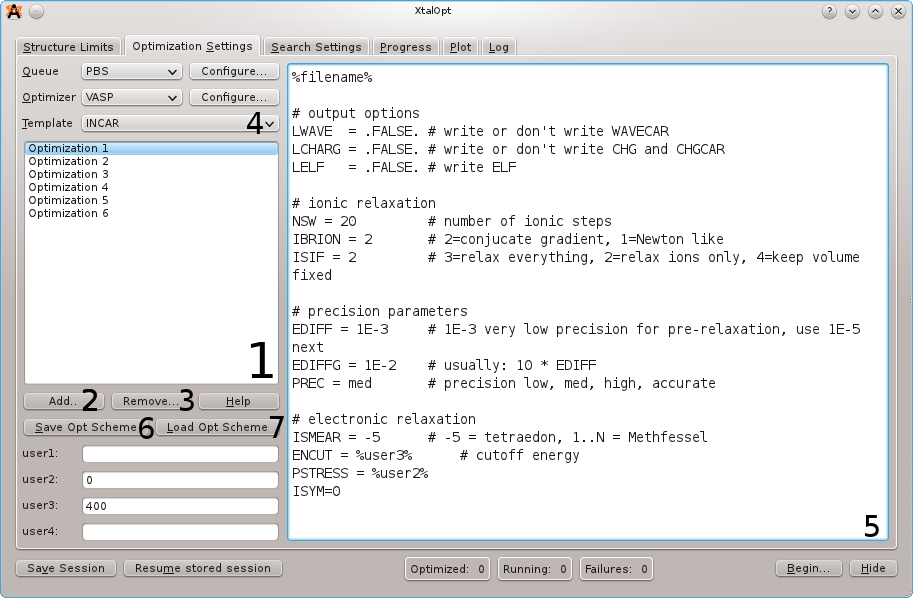
\includegraphics{optschemes-numberededitor.png}
\caption{width=}
\end{DoxyImage}


We will use the above screenshot as we describe the process of creating, saving, and loading optimization schemes. The numbers indicate\-:


\begin{DoxyEnumerate}
\item List of optimization steps
\item Button to add new optimization step
\item Button to remove current optimization step
\item Template selection menu
\item Template editor
\item Button to save current optimization scheme to file
\item Button to load optimization scheme from file
\end{DoxyEnumerate}\hypertarget{optschemes_gui-list}{}\subsection{Optimization step list}\label{optschemes_gui-list}
This list shows the currently available optimization steps in the order that they will be performed. The optstep that is currently selected for editing is highlighted, and the editable optstep can be selected by clicking the appropriate entry.\hypertarget{optschemes_gui-add}{}\subsection{Add new optimization step}\label{optschemes_gui-add}
Clicking this button will append a new optimization step to the optstep list. The new optstep's templates will be copies of the currently selected optstep's templates.\hypertarget{optschemes_gui-rem}{}\subsection{Remove current optimization step}\label{optschemes_gui-rem}
Click this button to delete the currently selected optimization step.\hypertarget{optschemes_gui-tselect}{}\subsection{Select template}\label{optschemes_gui-tselect}
This menu contains the filenames of the templates that are required by the currently selected queuing system (e.\-g. P\-B\-S, S\-G\-E, local...) and optimizer. The currently selected template is displayed in the template editor, and selecting a different template will update the editor.\hypertarget{optschemes_gui-editor}{}\subsection{Template editor}\label{optschemes_gui-editor}
This text editor is used to view and edit the currently selected template for the current optstep.\hypertarget{optschemes_gui-save}{}\subsection{Save scheme}\label{optschemes_gui-save}
This button will prompt for a location to save a .scheme file containing the current optimization step.\hypertarget{optschemes_gui-load}{}\subsection{Resume scheme}\label{optschemes_gui-load}
This button will prompt for an existing .scheme file to load.\hypertarget{optschemes_creating}{}\section{How to build an optimization scheme?}\label{optschemes_creating}
Creating a working scheme from scratch may take some time. We recommend checking the samples/ directory of the source code to obtain sample scheme for each optimizer (see \hyperlink{optschemes_loading}{How to load an optimization scheme?}) and verifying that they are appropriate for the system under consideration before starting a search.

If there is not an appropriate sample, the following prescription may be used to generate your own\-:


\begin{DoxyEnumerate}
\item Generate a random structure of the system under consideration. This may be done by hand, or by running a search just long enough to create the first random generation and saving one of the structures.
\item Create a starting optstep with the desired convergence criteria
\item Manually submit the optimization
\item If the optimization fails\-:
\begin{DoxyEnumerate}
\item First determine why -- if the maximum iterations were exceeded or the optimization was aborted due to a badly performing minimizer, try one of the ideas below. Other optimization problems are beyond the scope of this document.
\item Reduce the convergence criteria of the current trial optstep
\item Remove degrees of freedom, e.\-g. by fixing cell parameters, atomic positions, etc
\item Reduce the accuracy of the calculation in other ways (use a courser integration grid, etc).
\item Change the minimizer (e.\-g. tell the optimizer to use conjugate gradients rather than B\-F\-G\-S, etc)
\end{DoxyEnumerate}
\item Once the optimization succeeds, create another set of input files with the desired convergence criteria for all degrees of freedom.
\item Manually submit the new optimization step. If it fails, try the ideas above until it converges.
\item Once the structure has converged to the desired level of accuracy, try to optimize another randomly generated structure using the optsteps that succeeded previously. Refine them if needed.
\item Once you have successfully optimized enough random structures that you are confident in your method, gather all of the inputs used and write your scheme from them.
\end{DoxyEnumerate}

The scheme may be written by copying each input file into the template editor (with the appropriate optstep and template selected, of course) and replacing the structure-\/specific information with the appropriate keywords. Click the \char`\"{}\-Help\char`\"{} button for the complete list of keywords.

We have found that the optimization schemes are surprisingly transferable within an optimizer, so once you have a working optimization scheme for a given optimization code only minor tweaks (usually to the energy cutoffs, etc ) are necessary to use it on a different chemical system.\hypertarget{optschemes_saving}{}\section{How to save an optimization scheme for later?}\label{optschemes_saving}
Once you have written your optimization scheme, you will want to save it for fast retrieval later (otherwise you will need to copy/paste and edit all of the templates again!). To save, simply click the \char`\"{}\-Save Opt
\-Scheme\char`\"{} button and enter an appropriate filename with an extension of .scheme.\hypertarget{optschemes_loading}{}\section{How to load an optimization scheme?}\label{optschemes_loading}
Loading an optimization is quite simple -- just click the \char`\"{}\-Load Opt
\-Scheme\char`\"{} button and select the .scheme file you wish to load. This will also update the current queuing system and optimizer to those specified by the scheme.\hypertarget{optschemes_format}{}\section{What is saved?}\label{optschemes_format}
The optimization scheme files contain more than just the templates for each optstep. They also store queue and optimizer specific settings. This is useful for storing configuration options for different clusters along with the scheme. Note that although Xtal\-Opt will prompt for an S\-S\-H password if needed, it is {\bfseries N\-O\-T} stored in the scheme file.\hypertarget{optschemes_suggest}{}\section{Suggestions for optimization schemes}\label{optschemes_suggest}
\hypertarget{optschemes_sug-xtal}{}\subsection{Crystals (\-Xtal\-Opt)}\label{optschemes_sug-xtal}
The following list describes the optimization steps used in the samples/vasp-\/xtalopt.\-scheme file distributed with the Xtal\-Opt source code\-:
\begin{DoxyEnumerate}
\item Fix unit cell, only optimize atomic coordinates. A very loose convergence criterion is used, and the number of K\-P\-O\-I\-N\-Ts is kept small.
\item The cell volume is fixed, but atomic positions and cell parameters are allowed to vary. The convergence criteria is the same as before, as is the K\-P\-O\-I\-N\-T grid.
\item All degrees of freedom are considered using the same convergence criteria as before, but with a finer K\-P\-O\-I\-N\-T grid.
\item Same as before, but with a stricter convergence criteria.
\item Same as before, but with a stricter convergence criteria and more K\-P\-O\-I\-N\-Ts.
\item Same as before, but with more K\-P\-O\-I\-N\-Ts.
\end{DoxyEnumerate}

This is only one of many possible optimization schemes that may work for crystals. It may need to be modified to work for your particular system. 
%--- End generated contents ---

% Index
\backmatter
\newpage
\phantomsection
\clearemptydoublepage
\addcontentsline{toc}{section}{Index}
\printindex

\end{document}
